\documentclass[a4paper,12pt]{report}
\usepackage[latin1]{inputenc}   % Permet usar tots els accents i car�ters llatins de forma directa.
\usepackage[spanish]{babel}
%\decimalspanish{.}
\usepackage{latexsym}
\usepackage{hyperref}
\usepackage{theorem}
\usepackage{enumerate}
\usepackage{amsfonts, amscd, amsmath, amssymb}
\usepackage[pdftex]{graphicx}
\usepackage{epstopdf}
\usepackage{epsdice}

\newtheorem{definition}{Definici\'on}
\newtheorem{theorem}[definition]{Teorema}
\newtheorem{proposition}[definition]{Proposici\'on}
\newtheorem{corollary}[definition]{Corolario}
\newtheorem{lemma}[definition]{Lema}
\newtheorem{example}[definition]{Ejemplo}
\newtheorem{Rem}[definition]{Nota:}
\newcommand{\va}{variable aleatoria }
\def\N{I\!\!N}
\def\R{I\!\!R}
\def\Z{Z\!\!\!Z}
\def\Q{O\!\!\!\!Q}
\def\C{I\!\!\!\!C}
\decimalpoint


%\setlength{\textwidth}{15cm} \setlength{\textheight}{23cm}
\setlength{\textwidth}{17cm} \setlength{\textheight}{24cm}
%%\setlength{\textwidth}{15cm} \setlength{\textheight}{20cm}
\addtolength{\oddsidemargin}{-0.75cm}
\addtolength{\evensidemargin}{-0.75cm}
%\addtolength{\headheight}{\baselineskip}
\addtolength{\topmargin}{-1cm}
%\setlength{\topmargin}{0cm}
%\setlength{\footskip}{2.8cm}
\pagestyle{myheadings}

\title{ESTAD\'ISTICA APLICADA}
\date{}
\author{\large R. Alberich $\qquad \qquad$ J.L. Lisani}
\markboth{ESTAD\'ISTICA APLICADA curso 07-08}{ESTAD\'ISTICA APLICADA curso 07-08}
\makeindex

\begin{document}
\renewcommand{\tablename}{Tabla}
\renewcommand{\partname}{M\'odulo}

\maketitle

%\frontmatter
\tableofcontents
%\listoffigures
%\listoftables
\chapter*{Prefacio:\newline 
Estad\'istica en  Seguridad y Ciencias Policiales}


El enfoque racional de los problemas en cualquier �rea de las 
Ciencias implica un paso previo de recopilaci�n de datos y an�lisis
de los mismos que permite conocer en profundidad el problema
y eventualmente solucionarlo.

Ya sea para descubrir c�mo se mueven los planetas,
c�mo se desintegran los �tomos, c�mo distribuir el presupuesto 
municipal o c�mo asignar los recursos policiales para reducir 
la criminalidad, en el origen de la soluci�n est� la recopilaci�n 
de datos sobre el problema.
Las Ciencias Sociales, en las que se enmarcan las Ciencias Policiales 
y de Seguridad, no son ajenas a este m�todo de trabajo.

Sin embargo, los datos por s� solos poco aportan a la soluci�n 
de los problemas. Es su organizaci�n lo que permite descubrir
tendencias, singularidades, etc. que conduciran a la soluci�n.
La \textbf{Estad�stica Descriptiva} es la rama de las Matem�ticas que proporciona 
las t�cnicas necesarias para recopilar, organizar, representar, analizar e 
interpretar los datos.

En la mayor�a de ocasiones, y por razones pr�cticas,
el an�lisis estad�stico se hace sobre un 
conjunto de datos inferior al total disponible.
El ejemplo t�pico son las encuentas sobre intenci�n de voto, 
realizadas sobre unos pocos miles de personas que \textit{representan} 
al total de la poblaci�n. 
Los resultados obtenidos se generalizan despu�s a toda la poblaci�n.
La \textbf{Estad�stica In\-fe\-ren\-cial} permite conocer
el grado de fiabilidad de estas generalizaciones. 

En este curso estudiaremos las t�cnicas b�sicas de la Estad�stica Descriptiva
e Inferencial, de modo que aprenderemos a organizar y analizar 
conjuntos de datos y a conocer el grado de fiabilidad de las generalizaciones
realizadas a partir de ellos.

\vskip 0.5 cm
El curso se organiza en tres m�dulos:

\begin{enumerate}
\item El m�dulo I da una introducci�n a la notaci�n habitual de la
estad�stica y presenta las t�cnicas b�sicas de la Estad�stica Descriptiva.

\item En el m�dulo II se avanza en el estudio de la Estad�stica
Descriptiva y se dan los fundamentos de Probabilidad necesarios
para la Estad�stica Inferencial.

\item El m�dulo III se dedica al estudio de la Estad�stica Inferencial
\end{enumerate}

 
  

%\mainmatter
\part{}

El m�dulo I define los conceptos b�sicos de la Estad�stica Descriptiva
y presenta las t�cnicas b�sicas para la organizaci�n, representaci�n
y an�lisis de los datos estad�sticos.

Las definiciones te�ricas se acompa�an de m�ltiples ejemplos para facilitar
la comprensi�n. Asimismo, se explica c�mo resolver los problemas con
la ayuda de aplicaciones inform�ticas y c�mo acceder a bases de datos
estad�sticos oficiales.
 

\chapter{El lenguaje de la estad�stica}

En m\'ultiples �mbitos de las Ciencias o la Gesti�n es necesario
el estudio de temas relacionados con cada disciplina.
Por ejemplo:
\begin{itemize}
\item un experto en Seguridad puede estar interesado en estudiar
la criminalidad en una ciudad;
\item  un Economista, el nivel de paro de un pa�s;
\item un Ecologista, la deforestaci\'on de la selva amaz\'onica;
\item un F\'\i sico, la desintegraci\'on de elementos radioactivos en una central nuclear;
\item un Ingeniero, la calidad de las piezas producidas en una f�brica, etc.
\end{itemize}

Sea cual sea el tema a estudiar, la informaci\'on acerca del mismo
se obtiene realizando m\'ultiples \textbf{observaciones} de algunas de 
sus caracter\'isticas. Estas observaciones proporcionan una serie de \textbf{datos} 
que son organizados, analizados e interpretados usando unas t\'ecnicas estad\'\i sticas
comunes.

Antes de comenzar a explicar cualquier t\'ecnica estad\'istica es necesario
definir algunos conceptos b\'asicos y un vocabulario estad\'istico elemental. 
Entre otros aspectos, en este tema estudiaremos las nociones de poblaci\'on y muestra, la
diferencia entre estad\'istica descriptiva e inferencial y las distinci\'on
entre datos y variables.


\section{Poblaci�n y muestra}
El t\'ermino \textbf{poblaci\'on} hace referencia al conjunto total de \textit{elementos}
objeto del estudio estad\'istico. Por ejemplo:
\begin{itemize}
\item el n\'umero total de personas v\'ictimas de un delito, en un estudio sobre la criminalidad;
\item el n\'umero de personas en paro, en un estudio sobre el desempleo;
\item el n\'umero de \'arboles talados en el \'ultimo a\~no, en un estudio sobre la de\-fo\-res\-taci\'on;
\item el n\'umero de part\'iculas subat\'omicas generadas por un reactor nuclear, en un estudio
sobre la desintegraci\'on de elementos radiaoctivos;
\item el n\'umero de piezas defectuosas fabricadas, en un estudio sobre la ca\-li\-dad de la producci\'on.  
\end{itemize}

En la mayor\'ia de ocasiones es demasiado dif\'icil, caro o imposible obtener informaci\'on de 
todos los elementos de la poblaci\'on, por lo que el estudio estad\'istico se realiza
sobre un subconjunto de la poblaci\'on. Este subconjunto se denomina \textbf{muestra}.

Como veremos en el apartado siguiente, es frecuente que se deseen extraer conclusiones
relativas a la poblaci\'on total a partir de los datos de la muestra. Para que estas 
conclusiones sean fiables es necesario que la muestra sea \textbf{representativa} de 
la poblaci\'on. Se considera que si los elementos de la muestra han sido
elegidos al azar entre toda la poblaci\'on (\textbf{muestra aleatoria simple}), 
se obtiene una muestra representativa, aunque hay otras formas de tomar muestras. 
Otro factor a tener en cuenta es el tama\~no 
de la muestra, cuanto mayor sea mejor representar\'a al conjunto de la poblaci\'on.


\section{Tipos de estad�sticas: descriptiva e inferencial}
Tradicionalmente la disciplina de Estad\'istica se dividide en dos ramas:
descriptiva e inferencial. 

\vskip 0.2cm
La Estad\'istica Descriptiva tiene por objeto la descripci\'on de los 
datos recopilados, para ello proporciona t�cnicas que permiten:
\begin{itemize}
\item la \textbf{organizaci�n} de los datos mediante tablas y  representaciones gr�ficas;
\item el \textbf{an�lisis} de los datos mediante el c\'alculo de valores representativos 
como son las medidas de tendencia central y  de dispersi�n.
\end{itemize}


\vskip 0.2cm
La Estad\'istica Inferencial parte de los datos obtenidos a partir de una
muestra e intenta extraer conclusiones de las caracter\'\i sticas generales
de toda la poblaci\'on. Tambi\'en proporciona m\'etodos para medir la
fiabilidad de las conclusiones obtenidas y relacionar esta fiabilidad con
el tama\~no de la muestra estudiada.


\vskip 0.3 cm
Por ejemplo, en el caso del experto en Seguridad que hace un estudio sobre
la criminalidad en una ciudad, la manera de hacer el estudio puede ser la
siguiente:
\begin{enumerate}
\item En lugar de recopilar los datos relativos a los delitos cometidos
en toda la ciudad, recoge los datos de unos pocos barrios (elegidos
al azar o siguiendo alg\'un criterio determinado);
\item Organiza y analiza los datos recogidos utilizando t\'ecnicas de 
estad\'istica des\-crip\-ti\-va;
\item Utiliza t\'ecnicas de estad\'istica inferencial para generalizar
los resultados obtenidos a toda la ciudad y estimar el grado de fiabilidad
de esta generalizaci\'on.
\end{enumerate}


\section{Datos y variables}

Los \textbf{datos} se definen como las unidades de informaci\'on recopiladas
al hacer un estudio estad\'istico. Una \textbf{variable} es una caracter\'\i stica
o atributo que permite clasificar en diferentes categor\'\i as 
los elementos de la muestra o poblaci\'on en funci\'on de los
datos recopilados. 
Por ejemplo, el conjunto de personas v\'ictimas de un crimen se puede 
clasificar en funci\'on del sexo de las personas (hombre/mujer), la edad 
(menores de 20 a\~nos, entre 20 y 50, mayores de 50), etc. Cada uno 
de estos atributos (sexo, edad, etc.) es una variable.

Existen distintos tipos de variables que se pueden clasificar siguiendo 
tres criterios:

\begin{itemize}
\item Tipo de dato
\begin{itemize}
\item Nominales (cualitativas o de atributos):  cuando los datos no son num\'ericos 
y la comparaci�n entre sus valores s�lo puede ser de igualdad o desigualdad.

Por ejemplo: sexo, color de los ojos, afiliaci�n pol�tica, lugar de residencia, etc,...
\item Ordinales: cuando los datos no son num�ricos pero la
comparaci�n entre ellos establece un orden.

Por ejemplo: estado de �nimo (valores posibles: depresivo, normal y euf�rico ), estudios
(valores posibles: ninguno, primarios, secundarios, su\-pe\-rio\-res), etc...
\item Cuantitativas: cuando los datos son
num�ricos. Dentro de las variables cuantitativas hay dos tipos m�s
\begin{itemize}
\item Discretas:  cuando entre dos posibles valores no hay otro.
Por ejemplo: n�mero de  hijos de una familia, n�mero de letras de una palabra en un
texto, etc,...
\item Continuas:  cuando  entre dos posibles valores, siempre podemos encontrar otro valor
posible. Por ejemplo: altura, intereses de una cuenta bancaria, etc,...
\end{itemize}
\end{itemize}
\item Dimensi�n
\begin{itemize}
\item Unidimensionales: si s�lo se considera una �nica
caracter�stica.

Ejemplos: altura, edad, etc,...
\item Multidimensionales: si se consideran conjuntamente varias
caracter�sticas.

Ejemplos: edad y altura, altura y peso, edad, altura y sexo, etc,...
\end{itemize}
\item Tiempo
\begin{itemize}
\item Atemporales:
cuando los datos no est�n referidos, o no se con\-si\-de\-ra, el momento de tiempo en el que
fueron obtenidos.

Ejemplos: color de los ojos de cierto conjunto de individuos, peso de los  estudiantes del
curso de Estad\'istica, etc,...
\item Temporales o series cronol�gicas: en caso contrario.

Ejemplos: P.I.B. anual de Espa\~{n}a durante el periodo 1980 hasta 2004, n�mero de turistas
llegados al aeropuerto de  Palma durante los a\~{n}os 1970 al 2004, etc,...
\end{itemize}
\end{itemize}




\section{Ejercicios propuestos}


\noindent
\textbf{Ejercicio 1} 

Identificar la poblaci\'on y la muestra estudiados 
en los siguientes casos:
\begin{enumerate}[a)]
\item En un estudio sobre el consumo de drogas en un instituto se hace
una encuesta al $30\%$ por ciento de los alumnos de $2^\text{o}$ de 
bachillerato.
\item En un estudio sobre el consumo de drogas entre los j\'ovenes de
Ciutadella (menores de 35 a\~nos) se entrevista al $10\%$ de los clientes 
de los principales locales de copas.
\item En un estudio a nivel nacional sobre la influencia del alcohol 
en los accidentes de tr\'afico se realizan 10.000 controles de alcoholemia
en diferentes carreteras del pa\'is.
\end{enumerate}

\vskip 0.2 cm
\noindent
\textbf{Ejercicio 2} 

Decidir si para estudiar los siguientes casos se utilizan
herramientas de estad\'istica descriptiva o inferencial:
\begin{enumerate}[a)]
\item Un profesor de universidad debe proporcionar a su jefe de Departamento
un informe sobre el n\'umero de alumnos matriculados y sus calificaciones 
en el periodo 2005-2007. Para ello utilizar\'a estad\'istica ............... .
\item Una empresa desea conocer los h\'abitos de trabajo de sus trabajadores.
Para ello les hace rellenar una encuesta sobre sus horas de llegada y salida,
tiempo dedicado a responder el tel\'efono o el correo electr\'onico, 
tiempo dedicado a reuniones de trabajo con los jefes u otros compa\~neros, etc.
Los datos obtenidos se organizar\'an y analizar\'an usando estad\'istica ............. .
\item La Direcci\'on General de Tr\'afico desea evaluar la eficiencia a nivel
nacional de
la \'ultima campa\~na de prevenci\'on de accidentes a partir de los 
datos en una serie de municipios. Para ello utilizar\'a
herramientas de la estad\'istica ................ . 
\end{enumerate}

\vskip 0.2 cm
\noindent
\textbf{Ejercicio 3} 

Identificar al menos tres variables que pueden aparecer
en los siguientes estudios estad\'isticos:
\begin{enumerate}[a)]
\item Consumo de drogas en una ciudad.
\item Satisfacci\'on laboral de los empleados de una empresa.
\item Notas obtenidas por los alumnos de una asignatura. 
\end{enumerate}

\vskip 0.2 cm
\noindent
\textbf{Ejercicio 4} 

Clasificar las siguientes variables seg\'un su tipo,
dimensi\'on y nivel temporal:
\begin{enumerate}[a)]
\item N\'umero de personas que han sufrido un accidente de tr\'afico en los \'ultimos 5 a\~nos.
\item Nivel profesional de un militar (por ejemplo: soldado, cabo, sargento, etc.).
\item N\'umero de goles conseguidos por un jugador de f\'utbol a lo largo de la temporada 2006-07. 
\item Religi\'on de un individuo (por ejemplo: cat\'olico, musulm\'an, budista, etc.).
\item El peso y la altura de las participantes en un desfile de moda.
\item Cantidad de dinero gastada por una Administraci\'on en obras p\'ublicas a lo largo del \'ultimo a\~no. 
\end{enumerate}


%\section{Soluciones de los ejercicios}
%
%\noindent
%\textbf{Ejercicio 1}
%\begin{enumerate}[a)]
%\item Poblaci\'on: el total de los alumnos del instituto. 
%Muestra: el $30\%$ por ciento de los alumnos de $2^\text{o}$ de bachillerato
%\item Poblaci\'on: los habitantes de Ciutadella menores de 35 a\~nos.
%Muestra: el $10\%$ de los clientes de los principales locales de copas.
%\item Poblaci\'on: todos los conductores del pa\'is. Muestra: 10.000 conductores.
%\end{enumerate}
%
%\vskip 0.2 cm
%\noindent
%\textbf{Ejercicio 2}\begin{enumerate}[a)]
%\item Descriptiva.
%\item Descriptiva.
%\item Inferencial.
%\end{enumerate}
%
%\vskip 0.2 cm
%\noindent
%\textbf{Ejercicio 3}
%\begin{enumerate}[a)]
%\item Sexo, edad, nivel de estudios, nivel de ingresos, etc.
%\item Sexo, edad, antig\"uedad en la empresa, categor\'ia profesional, salario, etc.
%\item Tiempo dedicado al estudio, compaginaci\'on de estudios
%y trabajo, n\'umero de veces que se ha cursado la asignatura, 
%nota en los examenes de acceso a la universidad, etc.
%\end{enumerate}
%
%\vskip 0.2 cm
%\noindent
%\textbf{Ejercicio 4}
%\begin{enumerate}[a)]
%\item Cuantitativa discreta, unidimensional, temporal.
%\item Ordinal, unidimensional, atemporal.
%\item Cuantitativa discreta, unidimensional, temporal.
%\item Nominal, unidimensional, atemporal.
%\item Cuantitativa continua, multidimensional (bidimensional), atemporal.
%\item Cuantitativa continua, unidimensional, temporal.
%\end{enumerate}
%
%


\documentclass{article}
\usepackage[catalan]{babel}
\usepackage[latin1]{inputenc}   % Permet usar tots els accents i car�ters llatins de forma directa.
\usepackage{enumerate}
\usepackage{amsfonts, amscd, amsmath, amssymb}
\usepackage[pdftex]{graphicx}

\setlength{\textwidth}{16cm}
\setlength{\textheight}{24.5cm}
\setlength{\oddsidemargin}{-0.3cm}
\setlength{\evensidemargin}{0.25cm} \addtolength{\headheight}{\baselineskip}
\addtolength{\topmargin}{-3cm}

\newcommand\Z{\mathbb{Z}}
\newcommand\R{\mathbb{R}}
\newcommand\N{\mathbb{N}}
\newcommand\Q{\mathbb{Q}}
\newcommand\K{\Bbbk}
\newcommand\C{\mathbb{C}}

\newcounter{exctr}
\newenvironment{exemple}
{ \stepcounter{exctr} 
\hspace{0.2cm} 
\textit{Exemple  \arabic{exctr}: }
\it
\begin{quotation}
}{\end{quotation}}


\begin{document}

\textbf{\Large Tema 2.Sistemes}

\vskip 0.3 cm
\noindent
S'anomena \textbf{sistema} a qualsevol dispositiu o algoritme que modifica un senyal (entrada) 
per obtenir-ne un nou senyal (sortida) seguint alguna regla ben definida
(\'es a dir, no es tracta d'una modificaci\'o aleat\`oria del senyal).

\vskip 0.2 cm
\noindent
\textbf{Notaci\'o}. Per denotar que un sistema ${\cal T}$ transforma un senyal d'entrada $x$ 
en un senyal de sortida $y$ ho podem fer de 3 maneres:

\vskip 0.2 cm
\begin{center}
\begin{tabular}{ccccc}
1) 
\begin{minipage}{5cm}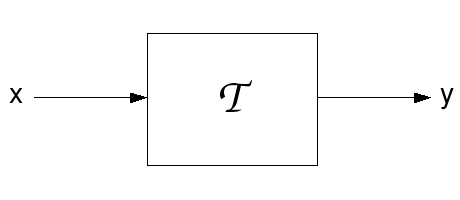
\includegraphics[width=5cm]{notaciosistema.png}\end{minipage} & &
2) $x \xrightarrow{{\cal T}} y $ & & 3) $y={\cal T}(x)={\cal T} \, x$ \\
(diagrama de blocs) & & & & 
\end{tabular}
\end{center}
\vskip 0.2 cm


\vskip 0.2 cm
\noindent
Exemples de sistemes:
\begin{itemize}
\item Acumulador

\begin{tabular}{lr}
$y[n]=y[n-1]+x[n]$ &
\begin{minipage}{5cm}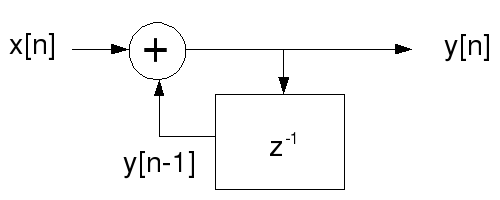
\includegraphics[width=5cm]{acumulador.png}\end{minipage}
\end{tabular}

\vskip 0.2 cm
\noindent
De manera equivalent es pot escriure: $y[n]=\sum_{k=-\infty}^n x[k]$

\item Diferenciador

\begin{tabular}{lr}
$y[n]=x[n-1]-x[n]$ &
\begin{minipage}{5cm}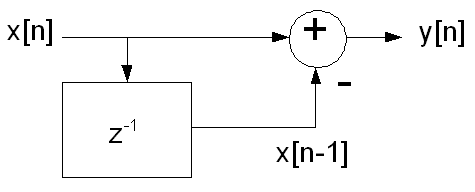
\includegraphics[width=5cm]{diferenciador.png}\end{minipage}
\end{tabular}

\item $y[n]=\mathrm{max}(x[n], x[n-1])$

\end{itemize}

\vskip 0.3 cm
\noindent
\textbf{Classificaci\'o dels sistemes}
\begin{itemize}

\item Sistemes lineals i no lineals.
Un sistema ${\cal T}$ es diu \textbf{lineal} si verifica que
\[
{\cal T}(ax_1[n]+bx_2[n])=a {\cal T}(x_1[n]) + b {\cal T}(x_2[n])
\]
\noindent
per a qualsevol parell de senyals d'entrada $x_1[n]$ i $x_2[n]$ i qualssevol
escalars $a$ i $b$.

\noindent
Si un sistema ${\cal T}$  \'es lineal llavors els seg\"uents diagrames de blocs 
s\'on equivalents:

\vskip 0.2 cm
\begin{center}
\begin{tabular}{ccc}
\begin{minipage}{6cm}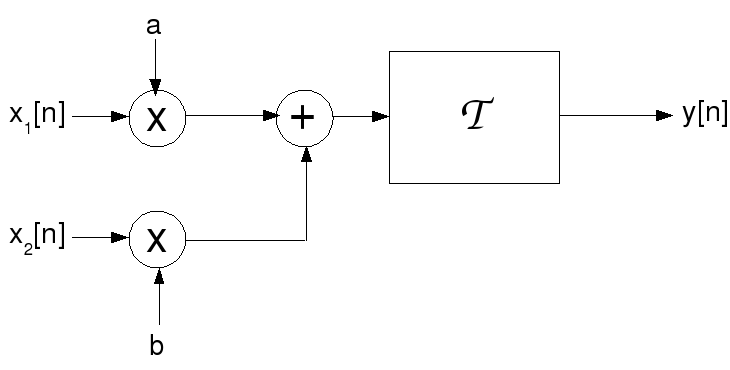
\includegraphics[width=6cm]{lineal1.png}\end{minipage}
 & $\qquad$ &
\begin{minipage}{6cm}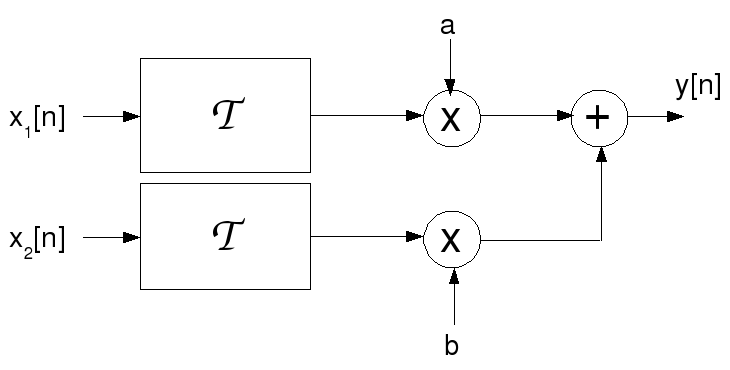
\includegraphics[width=6cm]{lineal2.png}\end{minipage}
\end{tabular}
\end{center}


\noindent
Exemples:
\begin{center}
\begin{tabular}{|c|c|}
 lineals & no lineals \\ \hline
$y[n]=Ax[n]$ & $y[n]=Ax[n]+B$ \\ & \\
$y[n]=nx[n]$ & $y[n]=nx[n]+B$ \\ & \\
$y[n]=x[n^2]$  & $y[n]=x^2[n]$ \\ & \\
$y[n]=e^n x[n]$ & $y[n]=e^{x[n]}$
\end{tabular}
\end{center}

\vskip 0.2cm
\noindent
Propietat dels sistemes lineals (\textbf{principi de superposici\'o}):
\[
{\cal T}(\sum_{k=1}^M a_k x_k[n]) =  \sum_{k=1}^M a_k y_k[n]
\]
\noindent
on $y_k[n]={\cal T} x_k[n]$, $(k=1, \cdots, M$.


\item Sistemes variants i invariants en el temps.
Un sistema es diu \textbf{invariant en el temps} si
a una entrada retardada en el temps li correspon una
sortida amb el mateix retard temporal. \'Es a dir:
\[
\text{si } y[n]={\cal T}(x[n]) \qquad \text{llavors} \qquad
y[n-k]={\cal T}(x[n-k])
\]

\noindent
Si un sistema ${\cal T}$  \'es invariant en el temps llavors els seg\"uents diagrames de blocs 
s\'on equivalents:

\vskip 0.2 cm
\begin{center}
\begin{tabular}{ccc}
\begin{minipage}{6cm}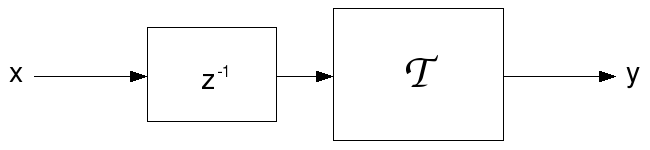
\includegraphics[width=6cm]{tinvariant1.png}\end{minipage}
 & $\qquad$ &
\begin{minipage}{6cm}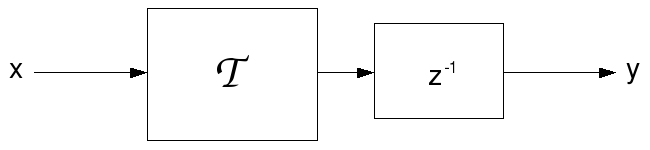
\includegraphics[width=6cm]{tinvariant2.png}\end{minipage}
\end{tabular}
\end{center}

\noindent
Exemples:
\begin{center}
\begin{tabular}{|c|c|}
 invariants en temps & no invariants \\ \hline
 $y[n]=x[n]-x[n-1]$ & $y[n]=nx[n]$  \\ & \\
 $y[n]=Ax[n]+B$ &  $y[n]=x[-n]$
\end{tabular}
\end{center}

\item Sistemes causals i no causals. Un sistema es diu \textbf{causal} si la seva
sortida en l'instant $n$ no depen de les entrades en els instants de temps
$n+1, n+2, \cdots$.

\noindent
Exemples:
\begin{center}
\begin{tabular}{|c|c|}
 causals & no causals \\ \hline
$y[n]=x[n]+x[n-5]$ & $y[n]=x[n]+x[n+5]$ \\ & \\
$y[n]=ax[n]$  & $y[n]=ax[-n]$ \\ & \\
$y[n]=x^2[n]$ & $y[n]=x[n^2]$ \\ & \\
$y[n]=3x[n]$ & $y[n]=3x[2n]$
\end{tabular}
\end{center}

\vskip 0.2 cm
\noindent
\textbf{Observaci\'o}: en sistemes que treballen en temps real 
(el processament es fa a mida que arriben els senyals d'entrada)
no \'es possible con\`eixer els valors futurs de l'entrada, per la qual cosa 
aquest sistemes nom\'es poden \'esser causals.

\item Sistemes estables i inestables.
Un sistema es diu \textbf{estable} si d\'ona sortides fitades a
entrades fitades.

\noindent
Exemples:
\begin{center}
\begin{tabular}{|c|c|}
 estables & inestables \\ \hline
$y[n]=ax[n]$ & $y[n]=\sum_{k=0}^\infty x[n-k]$ \\ & \\
$y[n]=\mathrm{max}\{ x[k] \, | \, k \leq n \}$  & $y[n]=x[n]+y^2[n-1]$ 
\end{tabular}
\end{center}


\item Sistemes est\`atics i din\`amics.
Un sistema es diu \textbf{est\`atic} o \textbf{sense mem\`oria} si la
seva sortida en l'instant $n$ no dep\`en de valors de l'entrada en instants
anteriors ni posteriors a $n$.

\noindent
Exemples:
\begin{center}
\begin{tabular}{|c|c|}
 est\`atics & din\`amics \\ \hline
$y[n]=ax[n]$ & $y[n]=x[n]+2x[n-1]$ \\ & \\
$y[n]=3nx[n]+ax^2[n]$ & $y[n]=\sum_{k=0}^n x[n-k]$ \\ & \\
$y[n]=5x[n]+2n$ & $y[n]=\sum_{k=0}^\infty x[n-k]$
\end{tabular}
\end{center}

\end{itemize}


\vskip 0.3 cm
\noindent
\textbf{Interconnexi\'o de sistemes}

\vskip 0.2 cm
\noindent
Els sistemes es poden interconnectar per a formar sistemes majors.
Les dues formes b\`asiques d'interconnectar dos sistemes s\'on:
\begin{itemize}
\item En \textbf{s\`erie} (o en \textbf{cascada}).
Donats dos sistemes ${\cal T}_1$ i ${\cal T}_2$, l'interconnexi\'o
en s\`erie de ${\cal T}_1$ i ${\cal T}_2$ d\'ona lloc a un nou sistema
${\cal T}_S$ tal que ${\cal T}_S={\cal T}_2 {\cal T}_1$, \'es a dir:
\[
{\cal T}_S(x[n])={\cal T}_2({\cal T}_1(x[n]))
\]
\noindent
gr\`aficament:

\begin{center}
\begin{minipage}{7cm}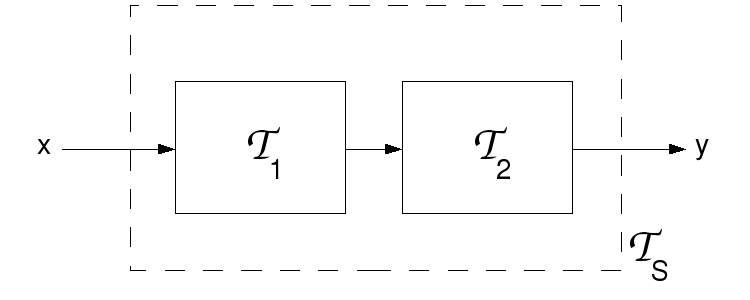
\includegraphics[width=7cm]{serie.png}\end{minipage}
\end{center}

\vskip 0.2cm
\noindent
Propietat: en general ${\cal T}_2 {\cal T}_1 \neq {\cal T}_1 {\cal T}_2$.

\item En \textbf{paral.lel}.
Donats dos sistemes ${\cal T}_1$ i ${\cal T}_2$, l'interconnexi\'o
en paral.lel de ${\cal T}_1$ i ${\cal T}_2$ d\'ona lloc a un nou sistema
${\cal T}_P$ tal que ${\cal T}_P={\cal T}_1 + {\cal T}_2$, \'es a dir:
\[
{\cal T}_P(x[n])={\cal T}_1(x[n]) + {\cal T}_2(x[n])
\]
\noindent
gr\`aficament:

\begin{center}
\begin{minipage}{6cm}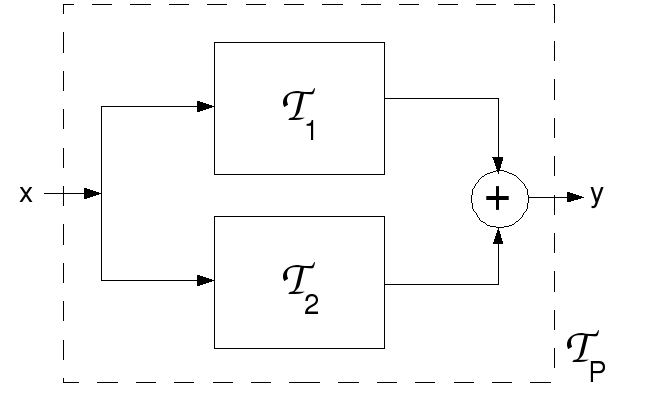
\includegraphics[width=6cm]{parallel.png}\end{minipage}
\end{center}

\vskip 0.2cm
\noindent
Propietat: ${\cal T}_1 + {\cal T}_2 = {\cal T}_2 + {\cal T}_1$.

\end{itemize}

\vskip 0.3 cm
\noindent
\textbf{An\`alisi de sistemes sineals i invariants en el temps (LTI)}
Els sistemes que s\'on a la vegada lineals i invariants en el temps es
denoten amb les sigles LTI (\textit{linear time-invariant}) i s\'on
especialment importants en Processament del Senyal perqu\`e
el seu funcionament es pot caracteritzar f\`acilment en funci\'o de la seva 
resposta a un senyal delta de Dirac.

\vskip 0.2 cm
\noindent
Sigui ${\cal T}$ un sistema LTI i sigui $x[n]$ un senyal d'entrada qualsevol.
Hem vist en el tema anterior que $x[n]$ es pot escriure en termes de la delta
de Dirac d'acord amb la f\`ormula $x[n]=\sum_{k=-\infty}^{+\infty} x[k] \delta[n-k]$,
de manera que la resposta del sistema a l'entrada $x[n]$ \'es:
\[
\begin{array}{ll}
y[n]& ={\cal T}(x[n])={\cal T} \left( \sum_{k=-\infty}^{+\infty} x[k] \delta[n-k] \right) = \\ \\
&= \text{(per linealitat)} = \sum_{k=-\infty}^{+\infty} x[k] {\cal T}(\delta[n-k]) = \\ \\
&= \text{(per invari\`ancia en el temps)}= \sum_{k=-\infty}^{+\infty} x[k] h[n-k]
\end{array}
\]
\noindent
on $h[n]={\cal T}(\delta[n])$, la resposta del sistema a una delta de Dirac.
$h[n]$ es coneix com \textbf{resposta impulsional del sistema}.

\vskip 0.2 cm
\noindent
Si observam el resultat anterior i recordam la definici\'o de convoluci\'o veurem que
\[
y[n]=x[n] * h[n]
\]

\noindent
\'Es a dir, \textbf{la sortida d'un sistema LTI \'es igual a la convoluci\'o
del senyal d'entrada per la resposta impulsional del sistema}. Per aquest motiu deim
que la resposta impulsional caracteritza totalment el sistema LTI. Si coneixem $h[n]$
podrem con\`eixer la resposta a qualsevol senyal d'entrada.

\vskip 0.2 cm
\noindent
Propietats dels sistemes LTI:
\begin{itemize}
\item Un sistema LTI \'es causal si i nom\'es si $h[n]=0 \quad \forall n < 0$.
\item Un sistema LTI \'es estable si  i nom\'es si $\sum_{n=-\infty}^{+\infty} |h[n]| < \infty$. 
\item La interconnexi\'o en s\`erie de dos sistemes LTI \'es commutativa, \'es a dir ${\cal T}_1 {\cal T}_2 = {\cal T}_2 {\cal T}_1$.
\end{itemize}


\vskip 0.2 cm
\noindent
Classificaci\'o dels sistemes LTI segons la duraci\`o de la seva resposta impulsional:
\begin{itemize}
\item Sistemes FIR (\textit{finite-duration impulsional response}).
S\'on aquells en qu\`e la resposta impulsional val zero fora d'un cert
interval de temps. En particular, per a un sistema FIR causal tenim que
\[
h[n]=0 \qquad \text{si } n < 0 \quad \text{i } n \geq M
\]
\noindent
per a algun valor de $M$ finit. De manera que la sortida d'aquest tipus de
sistemes es pot escriure com:
\[
y[n]=\sum_{k=0}^{M-1} x[k] h[n-k]=\sum_{k=0}^{M-1} x[n-k] h[k]
\]

\item Sistemes IIR (\textit{infinite-duration impulsional response}).
En aquest cas la resposta impulsional no s'anul.la fora de cap interval i
la sortida del sistema s'escriu com un sumatori infinit de valors.
\end{itemize}


\newpage
%\vskip 0.3 cm
\noindent
\textbf{Sistemes LTI descrits per equacions en difer\`encies finites}

\vskip 0.2 cm
\noindent
Els sistemes FIR s\'on \textit{realitzables} (es poden implementar amb un ordinador o circuit 
digital) ja que impliquen un nombre finit d'operacions i d'espais de mem\`oria.
En canvi, els sistemes IIR semblen irrealitzables ja que es necessiten, en principi,
infinites operacions i espai de mem\`oria. No obstant, hi ha un tipus de sistemes IIR, 
anomenats sistemes IIR \textbf{recursius} (o realimentats), que s\'on realitzables si involucren un nombre finit 
d'operacions.

En general, un sistema recursiu realitzable \'es aquell en qu\`e la seva sortida es pot escriure en funci\'o
d'un nombre finit de les entrades i de les sortides anteriors:
\[
y[n]=F( y[n-1], y[n-2], \cdots, y[n-N], x[n], x[n-1], \cdots, x[n-M]  )
\]

Un sistema es diu \textbf{no recursiu} si la seva sortida nom\'es dep\`en de les
entrades:
\[
y[n]=F( x[n], x[n-1], \cdots, x[n-M]  )
\]

Els sistemes FIR causals s\'on sistemes no recursius.


\vskip 0.3 cm
En aquest apartat estudiam com calcular de manera expl\'icita la sortida dels sistemes
recursius descrits per equacions de la forma:
\[
y[n]+\sum_{k=1}^N a_k y[n-k] = \sum_{k=0}^M b_k x[n-k]
\]
Aquest tipus d'equaci\'o rep el nom d'\textbf{equaci\'o en difer\`encies finites amb coeficients constants}.
$N$ s'anomena \textbf{grau} de l'equaci\'o.


\vskip 0.3 cm
La soluci\'o general d'aquesta equaci\'o es calcula de la forma seg\"uent:


\begin{enumerate}
\item la soluci\'o $y[n]$ s'escriu com la suma de dos termes
\[
y[n]=y_H[n]+y_P[n]
\]
\noindent
anomenats, respectivament, \textbf{soluci\'o homog\`enia} ($y_H$) i \textbf{soluci\'o particular} ($y_P$).

\item La soluci\'o homog\`enia \'es la soluci\'o de l'equaci\'o:
\[
y[n]+\sum_{k=1}^N a_k y[n-k] = 0
\]
\noindent
que rep el nom d'\textbf{equaci\'o homog\`enia}.

$y_H[n]$ es calcula de la seq\"uent manera:

\begin{enumerate}

\item escrivim l'\textbf{eq\"uaci\'o caracter\'istica} associada a l'eq\"uaci\'o
homog\`enia:
\[
\lambda^N+\sum_{k=1}^N a_k \lambda^{N-k} = 0
\]
\noindent
aquesta equaci\'o t\'e grau $N$.
\item calculam les arrels de l'eq\"uaci\'o caracter\'istica:
\[
\begin{array}{c}
\lambda_1 \text{ amb multiplicitat } r_1 \\ \\
\lambda_2 \text{ amb multiplicitat } r_2 \\ \\
\cdots \\ \\
\lambda_m \text{ amb multiplicitat } r_m
\end{array}
\]

\noindent
Es verifica que $r_1+r_2+\cdots+r_m=N$

\item per a cada arrel $\lambda_i$ amb multiplicitat $r_i$ de l'equaci\'o 
caracter\'istica tenim una soluci\'o parcial de l'equaci\'o homog\`enia:
\[
C_{i1} \lambda_i^n + C_{i2} n \lambda_i^n + \cdots + C_{i r_i} n^{r_i-1} \lambda_i^n
= \sum_{j=1}^{r_i} C_{ij} n^{j-1} \lambda_i^n
\]

\item la soluci\'o de l'equaci\'o homog\`enia s'obt\'e sumant totes les solucions parcials
\[
y_H[n]=\sum_{i=1}^m \sum_{j=1}^{r_i} C_{ij} n^{j-1} \lambda_i^n
\]

\item les constants $C_{ij}$ es calculen a partir de les 
\textbf{condicions inicials} del problema.

\end{enumerate}



\item La forma de la soluci\'o particular $y_P[n]$ dep\`en del tipus del senyal d'entrada $x[n]$:

\begin{tabular}{c|c}
Senyal d'entrada & Soluci\'o particular \\ 
$x[n]$, $n \geq 0$ & $y_P[n]$, $n \geq 0$ \\ 
($x[n]=0$ si $n < 0$) & ($y_P[n]=0$ si $n < 0$)\\  \hline \\
$(A_0+A_1 n + \cdots + A_k n^k) \alpha^n$ & $(B_0+B_1 n + \cdots + B_k n^k) n^M \alpha^n$ \\ \\
 & on $M$ \'es la multiplicitat de $\alpha$ com a soluci\'o de l'equaci\'o caracter\'istica \\
\hline
\\
$A \cos(\omega_0 n)$ & $B_1 \cos(\omega_0 n) + B_2 \sin(\omega_0 n)$ \\ \\
\hline
\\
$A \sin(\omega_0 n)$ & $B_1 \cos(\omega_0 n) + B_2 \sin(\omega_0 n)$ 
\end{tabular}

\noindent
\vskip 0.3 cm
Les constants $B_i$ es calculen per substituci\'o en l'equaci\'o en difer\`encies inicial.

\end{enumerate}



\vskip 0.4cm
\noindent
\textbf{Exemple:} Calculau la soluci\'o del sistema recursiu descrit per l'equaci\'o seg\"uent
considerant condicions inicials $y[k]=1$ per a tot $k < 0$.
\[
y[n]-5y[n-1]+6y[n-2]=u[n]
\]

\vskip 0.2cm
\noindent
Soluci\'o:
\begin{enumerate}
\item $y[n]=y_H[n]+y_P[n]$
\item $y_H[n]$:
\begin{enumerate}
\item equaci\'o homog\`enia: $y[n]-5y[n-1]+6y[n-2]=0$ (grau 2)
\item equaci\'o caracter\'istica: $\lambda^2 - 5 \lambda + 6 =0$
\item arrels de l'equaci\'o caracter\'istica: $3$ i $2$
\item $y_H[n]=C_1 3^n + C_2 2^n$
\end{enumerate}
\item $y_P[n]$:
\begin{enumerate}
\item $x[n]=A u[n]$, amb $A=1$ (polinomi de grau 0)
\item $y_P[n]=B u[n]$
\item substituint a l'equaci\'o inicial:
\[
\begin{array}{l}
y_P[n]=B u[n] \\
y_P[n-1]=B u[n-1] \\
y_P[n-2]=B u[n-2] \\
y_P[n]-5y_P[n-1]+6y_P[n-2]=u[n] \quad \Rightarrow Bu[n]-5Bu[n-1]+6Bu[n-2]=u[n]\\
\text{per a $n >= 2$ la resposta s'estabilitza i tenim:} \qquad B-5B+6B=1 \quad \Rightarrow B=\frac{1}{2}
\end{array}
\]
\item per tant: $y_P[n]=\frac{1}{2} u[n]$
\end{enumerate}

\item Soluci\'o completa: $y[n]=C_1 3^n + C_2 2^n+\frac{1}{2} u[n]$

\item C\`alcul de $C_1$ i $C_2$:
\begin{enumerate}
\item de l'equaci\'o inicial i aplicant les condicions inicials ($y[k]=1$ si $k < 0$):
\[
\begin{array}{l}
y[0]-5y[-1]+6y[-2]=u[0] \quad \longrightarrow \quad y[0]=5-6+1=0 \\
y[1]-5y[0]+6y[-1]=u[1] \quad \longrightarrow \quad y[1]=0-6+1=-5 
\end{array}
\]
\item de la soluci\'o trobada:
\[
\begin{array}{l}
y[0]=C_1 3^0 + C_2 2^0+\frac{1}{2} u[0] \quad \longrightarrow \quad y[0]=C_1+C_2+\frac{1}{2} \\ 
y[1]=C_1 3^1 + C_2 2^1+\frac{1}{2} u[1] \quad \longrightarrow \quad y[1]=3C_1+2C_2+\frac{1}{2} \\ 
\end{array}
\]
\item resolent el sistema d'equacions que plantejen les anteriors equacions: $C_1=-\frac{13}{2}$, $C_2=7$.

\end{enumerate}
 
\item Soluci\'o final: $y[n]=-\frac{13}{2} \cdot 3^n + 7 \cdot 2^n+\frac{1}{2} u[n]$

\end{enumerate}



\vskip 0.4cm
\noindent
\textbf{Respostes lliure i for\c{c}ada d'un sistema} 

\vskip 0.2 cm
\noindent
La resposta total d'un sistema es pot escriure com la suma de dos termes
\[
y[n]=y_{zi}[n]+y_{zs}[n]
\]

\noindent
on $y_{zi}$ s'anomena \textbf{resposta zero-input}, resposta lliure o resposta natural
del sistema. \'Es la resposta que s'obt\'e quan l'entrada \'es nul.la i coincideix amb
la soluci\'o homog\`enia de l'equaci\'o en difer\`encies ($y_{zi}[n]=y_H[n]$).

\noindent
$y_{zs}$ rep el nom de \textbf{resposta zero-state} o resposta for\c{c}ada del sistema
i \'es la resposta que s'obt\'e davant un senyal d'entrada quan les condicions inicials s\'on
nul.les (sistema en rep\`os o relaxat). Coincideix amb la soluci\'o del sistema
quan les condicions inicials s\'on nul.les ($y_{zs}[n]=y[n]$, amb $y[n]=0$ per $n < 0$).

\vskip 0.4cm
\noindent
\textbf{Resposta impulsional d'un sistema recursiu} 

\vskip 0.2 cm
\noindent
La resposta impulsional $h[n]$ d'un sistema LTI es defineix com la resposta
del sistema a un senyal delta de Dirac. En el cas d'un sistema descrit per una
equaci\'o en difer\`encies $h[n]$ coindideix amb la resposta del sistema quan
$x[n]=\delta[n]$ i les condicions inicials s\'on nul.les: 
\[
h[n]=y[n] \qquad \text{quan} \quad x[n]=\delta[n] \quad \text{i} \quad y[n]=0 \text{ per } n < 0
\]

\noindent
a m\'es, com $x[n]=\delta[n]$, resulta que $y_P[n]=0$ i per tant $y[n]=y_H[n]$.



\vskip 0.4cm
\noindent
\textbf{Estructures per a la realitzaci\'o de sistemes LTI descrits per equacions en difer�ncies} 

\vskip 0.2 cm
\noindent
El diagrama de blocs corresponent a l'equaci\'o en difer\`encies

\[
y[n]=-\sum_{k=1}^N a_k y[n-k] + \sum_{k=0}^M b_k x[n-k]
\]

\noindent
es mostra en la figura \ref{blocsLTI}-(a). Per la propietat 
conmutativa de la connexi\'o en s\`erie dels sistemes LTI
(${\cal T}_1 {\cal T}_2 = {\cal T}_2 {\cal T}_1$), aquest diagrama
\'es equivalent al de la figura \ref{blocsLTI}-(b), que
\'es equivalent al de la figura \ref{blocsLTI}-(c). En aquest 
darrer diagrama el nombre d'operacions de retard \'es menor que
en els diagrames anteriors, per la qual cosa es considera que
la realitzaci\'o del sistema \'es m\'es eficient. La realitzaci\'o de l'esquerra
s'anomena \textbf{forma directa} del sistema mentre que la de
la dreta es diu \textbf{forma can\`onica}.

\begin{figure}[htbp]
\begin{center}
\begin{tabular}{cc}
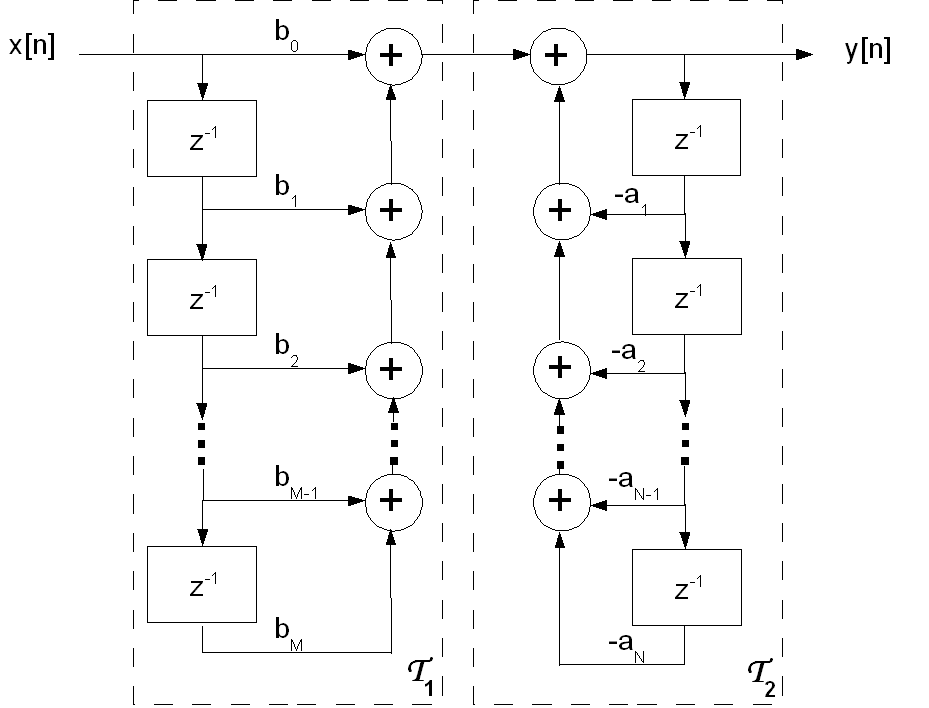
\includegraphics[width=8cm]{formadirecta.png} &
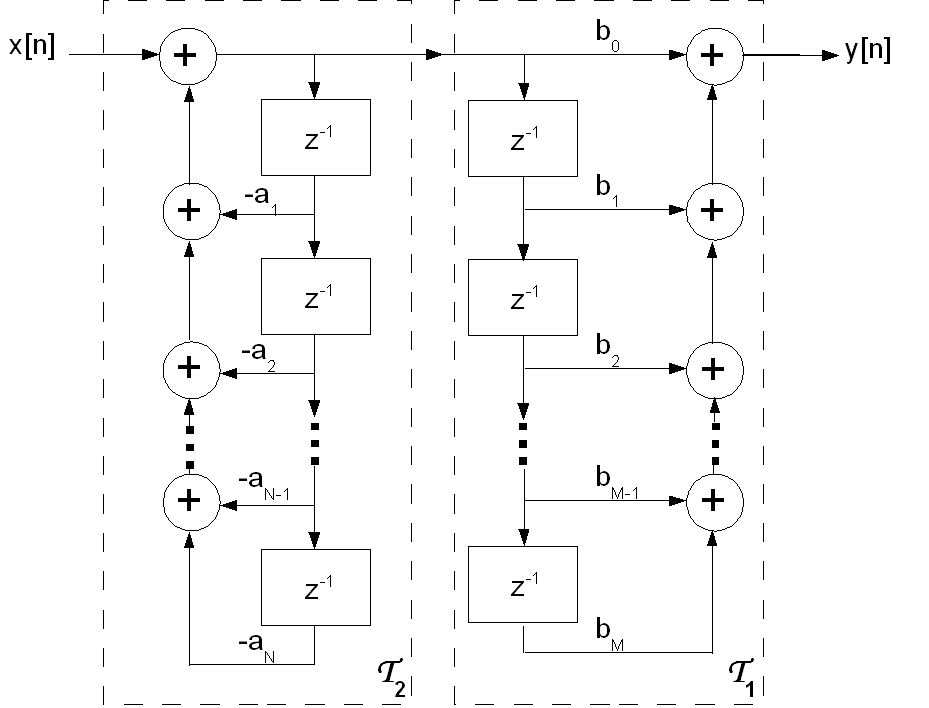
\includegraphics[width=8cm]{formacommutada.png} \\ \\
(a) & (b) 
\end{tabular}
\begin{tabular}{c}
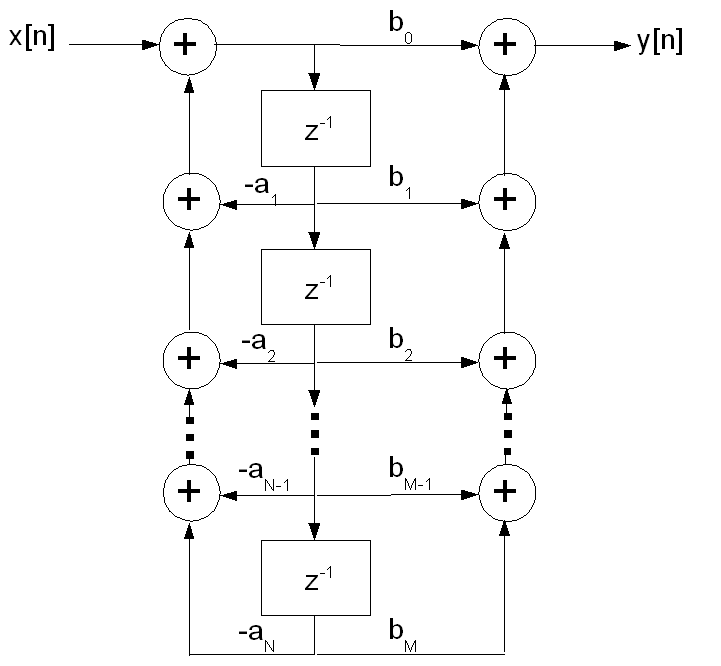
\includegraphics[width=7.5cm]{formacanonica.png} \\ \\
(c)
\end{tabular}
\end{center}
\caption{(a) forma directa. (b) commutaci\'o de les estructures
del diagrama anterior. (c) forma can\`onica.}
\label{blocsLTI}
\end{figure}


\end{document}



\documentclass{article}
\usepackage[catalan]{babel}
\usepackage[latin1]{inputenc}   % Permet usar tots els accents i car�ters llatins de forma directa.
\usepackage{enumerate}
\usepackage{amsfonts, amscd, amsmath, amssymb}
\usepackage[pdftex]{graphicx}
\usepackage{longtable}

\setlength{\textwidth}{16cm}
\setlength{\textheight}{24.5cm}
\setlength{\oddsidemargin}{-0.3cm}
\setlength{\evensidemargin}{0.25cm} \addtolength{\headheight}{\baselineskip}
\addtolength{\topmargin}{-3cm}

\newcommand\Z{\mathbb{Z}}
\newcommand\R{\mathbb{R}}
\newcommand\N{\mathbb{N}}
\newcommand\Q{\mathbb{Q}}
\newcommand\K{\Bbbk}
\newcommand\C{\mathbb{C}}

\newcounter{exctr}
\newenvironment{exemple}
{ \stepcounter{exctr} 
\hspace{0.2cm} 
\textit{Exemple  \arabic{exctr}: }
\it
\begin{quotation}
}{\end{quotation}}


\begin{document}

\textbf{\Large Tema 3.An\`alisi transformat (transformada Z)}

\vskip 0.2 cm

La transformada Z permet caracteritzar els sistemes digitals i estudiar, 
de manera relativament senzilla, algunes de les seves propietats (estabilitat, causalitat, etc.).

\vskip 0.3 cm
\noindent
\textbf{Transformada Z}

\vskip 0.2 cm
\noindent
Es defineix la transformada Z d'un senyal discret $x[n]$ com:
\[
X(z)={\cal Z} \{x[n]\})=\sum_{n=-\infty}^{+\infty} x[n] z^{-n}
\]

\noindent
on $z$ \'es una variable complexa. En funci\'o del valor de $z$ aquest sumatori pot 
\'esser infinit (s\`erie divergent). Anomenam \textbf{regi\'o de converg\`encia (ROC)}
el conjunt de valors de $z$ que fan que la s\`erie sigui convergent.

\vskip 0.5 cm
\noindent
Exemples:

\vskip 0.2 cm
\begin{tabular}{l|l|l}
$x[n]$ & $X(z)$ & ROC \\ \hline  & & \\
$\{\underline{1}, 2, 5, 7, 0, 1 \}$ & $1+2z^{-1}+5z^{-2}+7z^{-3}+z^{-5}$ &
pla $z$, excepte $z=0$ \\ \hline  & & \\
$\{1, 2, \underline{5}, 7, 0, 1 \}$ & $z^2+2z+5+7z^{-1}+z^{-3}$ &
pla $z$, excepte $z=0$ i $z=\infty$ \\ \hline  & & \\
$\delta[n]$ & $1$ & tot el pla $z$ \\ \hline  & & \\
$\delta[n-k]$ ($k > 0$) & $z^{-k}$ ($k > 0$) & pla $z$, excepte $z=0$ \\ \hline  & & \\
$\delta[n+k]$ ($k > 0$) & $z^{k}$ ($k > 0$) & pla $z$, excepte $z=\infty$ \\ \hline  & & \\
$(\frac{1}{2})^n u[n]$ & $\sum_{n=0}^{\infty} \left(\frac{1}{2} z^{-1} \right)^n=\displaystyle \frac{1}{1-\frac{1}{2}z^{-1}}$ &
$|z| > \frac{1}{2}$ \\ \hline  & & \\
$-(\frac{1}{2})^n u[-n-1]$ & $-\sum_{n=-\infty}^{1} \left( \frac{1}{2} z^{-1} \right)^n=\displaystyle \frac{1}{1-\frac{1}{2} z^{-1}}$ &
$|z| < \frac{1}{2}$ \\ \hline  & & \\
$2^n u[n] + 5^n u[-n-1]$ & 
$\sum_{n=0}^{\infty} \left(2 z^{-1} \right)^n + \sum_{n=-\infty}^{1} \left( 5 z^{-1} \right)^n=\frac{1}{1-2 z^{-1}} - \frac{1}{1-5 z^{-1}}$ &
$2 < |z| < 5$ \\ \hline 
\end{tabular}

\vskip 0.7 cm
\noindent
Observem que en els 5 primers exemples els senyals s\'on de duraci\'o finita mentre que els
4 darrers s\'on de duraci\'o infinita. En els primers casos la ROC \'es igual a tot el pla
excepte, possiblement, els punts $z=0$ i/o $z=\infty$.
En el cas dels senyals infinits la ROC, en general, t\'e la forma seg\"uent (forma d'anell):
$r_2 < |z| < r_1$, on $r_2$ i $r_1$ s\'on dos valors constants que depenen de la definici\'o de $x[n]$.

\vskip 0.5 cm
\noindent
Un senyal $x[n]$ queda totalment determinat per la seva transformada Z i la seva ROC. Con\`eixer
nom\'es la transformada Z no permet saber quin era el senyal original (veure exemples 6 i 7).

\vskip 0.5 cm
\noindent
Per als senyals causals ($x[n]=0$ si $n < 0$) la ROC t\'e la forma $|z| > r$, mentre per 
als no causals ($x[n]=0$ si $n \geq 0$) la ROC \'es de la forma $|z| < r$, per a alguna
constant $r$  (veure exemples 6 i 7).

\begin{figure}[htbp]
\begin{center}
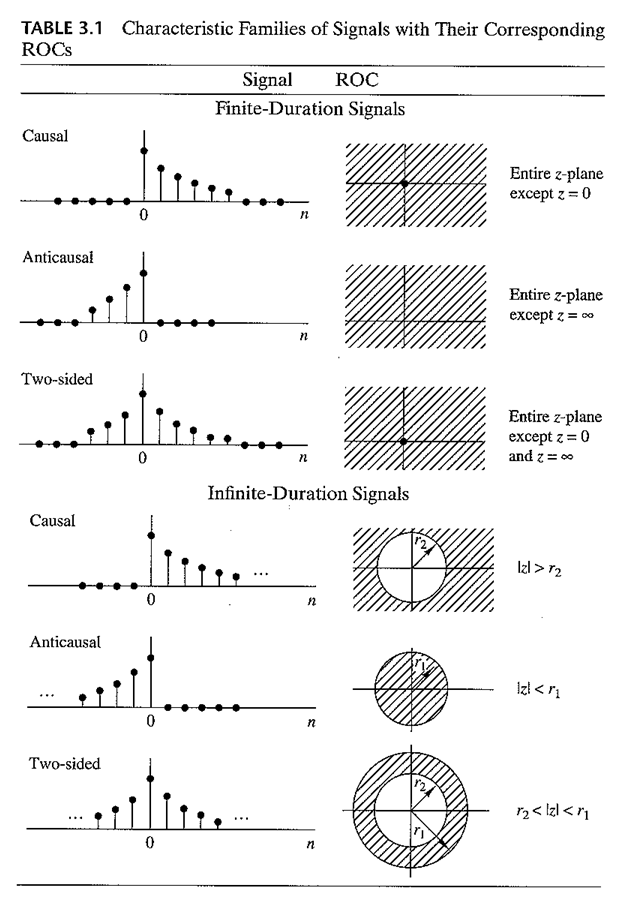
\includegraphics[width=12cm]{signalROC.png}
\end{center}
\caption{Font: Digital Signal Processing, J. Proakis, D. Manolakis, Pearson Prentice Hall, 2007}
\end{figure}

\newpage
%\vskip 0.3 cm
\noindent
\textbf{Propietats de la transformada Z}

\vskip 0.2 cm
\noindent
Denotam $X(z)={\cal Z} \{ x[n] \}$, amb ROC=$\text{ROC}_0 = r_2 < |z| < r_1$,
$X_1(z)={\cal Z} \{ x_1[n] \}$ amb ROC=$\text{ROC}_1$ i
$X_2(z)={\cal Z} \{ x_2[n] \}$ amb ROC=$\text{ROC}_2$.

\begin{enumerate}
\item Linealitat. 

\[
{\cal Z} \{ a_1 x_1[n] + a_2 x_2[n] \} = a_1 X_1(z) + a_2 X_2(z) 
\]

amb ROC=com a m\'inim, intersecci\'o de $\text{ROC}_1$ i $\text{ROC}_2$.

\item Despla\c{c}ament en temps.
\[
{\cal Z} \{ x[n-k] \} = z^{-k} X(z)
\]

amb ROC=$\text{ROC}_0$ excepte $z=0$ si $k > 0$ i $z=\infty$ si $k < 0$. 

\item Escalat.
\[
{\cal Z} \{ a^n x[n] \} = X(a^{-1} z) 
\]

amb ROC=$|a| r_2 < |z| < |a| r_1$.

\item Inversi\'o temporal.
\[
{\cal Z} \{ x[-n] \} = X(z^{-1}) 
\]

amb ROC=$\frac{1}{r_1} < |z| < \frac{1}{r_2}$.


\item Derivaci\'o en el domini $z$.
\[
{\cal Z} \{ nx[n] \} = -z \frac{d \, X(z) }{dz} 
\]

amb ROC=$\text{ROC}_0$.


\item Conjugaci\'o.
\[
{\cal Z} \{ x^*[n] \} = X^*(z^*) 
\]

amb ROC=$\text{ROC}_0$.

\item Convoluci\'o.
\[
{\cal Z} \{ x_1[n] * x_2[n] \} = X_1(z) X_2(z)
\]

amb ROC=com a m\'inim, intersecci\'o de $\text{ROC}_1$ i $\text{ROC}_2$.


\end{enumerate}

%\begin{figure}[htbp]
%\begin{center}
%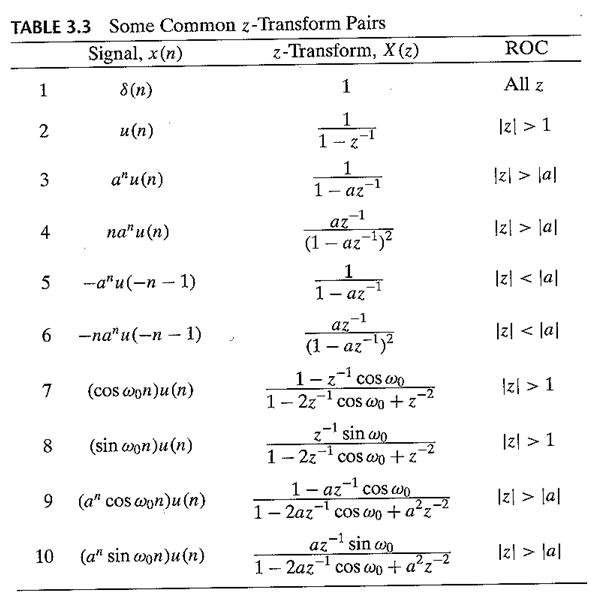
\includegraphics[width=12cm]{TZhabituals.png}
%\end{center}
%\caption{Font: Digital Signal Processing, J. Proakis, D. Manolakis, Pearson Prentice Hall, 2007}
%\end{figure}

\vskip 0.5cm
\noindent
\textbf{Transformades Z habituals}
\vskip 0.3 cm

\begin{tabular}{ccc}
\begin{tabular}{c|c|c}
$x[n]$ & $X(z)$ & ROC \\ \hline & &  \\
$\delta[n]$ & $1$ & tot $z$ \\ & & \\
$u[n]$ & $\frac{1}{1-z^{-1}}$ & $|z| > 1$ \\ & & \\
$a^nu[n]$ & $\frac{1}{1-az^{-1}}$ & $|z| > |a|$ \\ & & \\
$na^nu[n]$ & $\frac{az^{-1}}{(1-az^{-1})^2}$ & $|z| > |a|$ \\ & & \\
$-a^nu[-n-1]$ & $\frac{1}{1-az^{-1}}$ & $|z| < |a|$ 
\end{tabular}
&
$\qquad$
&
\begin{tabular}{c|c|c}
$x[n]$ & $X(z)$ & ROC \\ \hline & &  \\
$-na^nu[-n-1]$ & $\frac{az^{-1}}{(1-az^{-1})^2}$ & $|z| < |a|$ \\ & & \\
$\cos(\omega_0n) u[n]$ & $\frac{1-z^{-1}\cos \omega_0}{1-2z^{-1}\cos\omega_0+z^{-2}}$ & $|z|>1$ \\ & & \\
$\sin(\omega_0n) u[n]$ & $\frac{z^{-1}\sin \omega_0}{1-2z^{-1}\cos\omega_0+z^{-2}}$ & $|z|>1$ \\ & & \\
$(a^n\cos(\omega_0n)) u[n]$ & $\frac{1-az^{-1}\cos \omega_0}{1-2az^{-1}\cos\omega_0+a^2z^{-2}}$ & $|z|>|a|$ \\ & & \\
$(a^n\sin(\omega_0n)) u[n]$ & $\frac{az^{-1}\sin \omega_0}{1-2az^{-1}\cos\omega_0+a^2z^{-2}}$ & $|z|>|a|$ 
\end{tabular}
\end{tabular}


\newpage
\noindent
\textbf{Transformades Z racionals}

\vskip 0.3cm
\noindent
Un tipus important de transformades Z s\'on les transformada Z racionals,
que s'escriuen com a quocient de dos polinomis:

\begin{equation}
X(z)=\frac{P(z)}{Q(z)}=\frac{b_0+b_1z^{-1}+\cdots+b_Mz^{-M}}{a_0+a_1z^{-1}+\cdots+a_Nz^{-N}}=
\frac{b_0}{a_0} z^{N-M} \frac{(z-z_1)(z-z_2) \cdots (z-z_M)}{(z-p_1)(z-p_2) \cdots (z-p_N)}
\end{equation}

\vskip 0.3cm
\noindent
\textbf{Pols i zeros de la transformada Z}. S'anomenen \textbf{zeros} de $X(z)$ els valors de $z$ que fan
que $X(z)=0$. S'anomenen \textbf{pols} de $X(z)$ els valors de $z$ que fan que $X(z)=\infty$. 


\vskip 0.3cm
\noindent
Amb la factoritzaci\'o de l'equaci\'o anterior, $z_1, z_2, \cdots, z_M$ s\'on zeros de la transformada racional
i $p_1, p_2, \cdots, p_N$ s\'on pols. A m\'es, si $N > M$, $z=0$ \'es zero de $X(z)$ (amb multiplicitat $N-M$) 
i si $N < M$, $z=0$ \'es pol de $X(z)$ (amb multiplicitat $M-N$). Si els polinomis $P(z)$ i $Q(z)$ tenen arrels
en com\'u llavors haur\`a zeros i pols que es cancel.laran mutuament.

\vskip 0.3cm
\noindent
A $\infty$ existeix un zero si $X(\infty)=0$ i hi existeix un pol si $X(\infty)=\infty$. Si comptam els zeros
i pols a $\infty$, $X(z)$ t\'e el mateix nombre de pols i zeros.

\vskip 0.3cm
\noindent
Els pols i els zeros de $X(z)$ es representen en un \textbf{diagrama de zeros i pols}. La ROC de $X(z)$ no
cont\'e cap pol.

\vskip 0.3cm
\noindent
Exemples:

\begin{tabular}{l|c}
 & diagrama pols-zeros \\ \hline &  \\
 
\begin{tabular}{l}
$x[n]=a^n u[n] \qquad (a > 0)$ \\ \\
$X(z)=\frac{1}{1-az^{-1}}=\frac{z}{z-a}$ \\ \\
$\text{ROC:  } |z| > |a|$ \\ \\
$\text{zeros:  } z_1=0$ \\ \\
$\text{pols:  } p_1=a $
\end{tabular}


&

\begin{minipage}{5cm} 
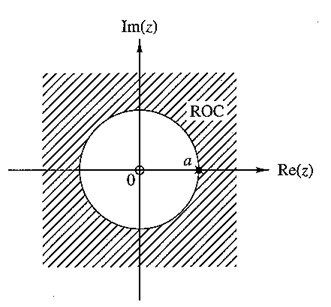
\includegraphics[width=5cm]{ex1PolsZeros.png}
\end{minipage} \\ \hline & \\

\begin{tabular}{l}
$x[n]=\begin{cases}a^n & \text{si } 0 \leq n \leq M-1 \\ $0$ & \text{altrament} \end{cases} \, (a>0, \text{real})$\\ \\ 
$X(z)=\frac{z^M-a^M}{z^{M-1}(z-a)}$ \\ \\
$\text{ROC:  } z \neq 0$ \\ \\
$\text{zeros:  } z_i=ae^{j 2\pi k/M}, \qquad i=1,\cdots, M-1$\\ \\
$\text{pols:  } p=0 \,\, \text{(multiplicitat $M-1$)}$
\end{tabular}


&

\begin{minipage}{5cm} 
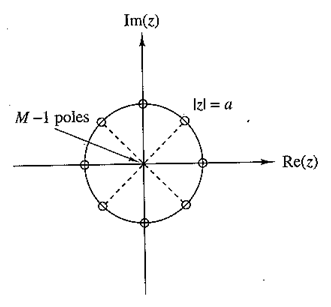
\includegraphics[width=5cm]{ex2PolsZeros.png}
\end{minipage} (M=8)

\end{tabular}


\newpage
\noindent
\textbf{Posici\'o dels pols i estabilitat de senyals causals reals}

\vskip 0.2 cm
\noindent
\textbf{Cas 1}. Senyal real amb un \'unic pol: $x[n]=a^nu[n]$, $X(z)=\frac{1}{1-az^{-1}}$, ROC=$|z|>|a|$, ($a$ real)
\begin{center}
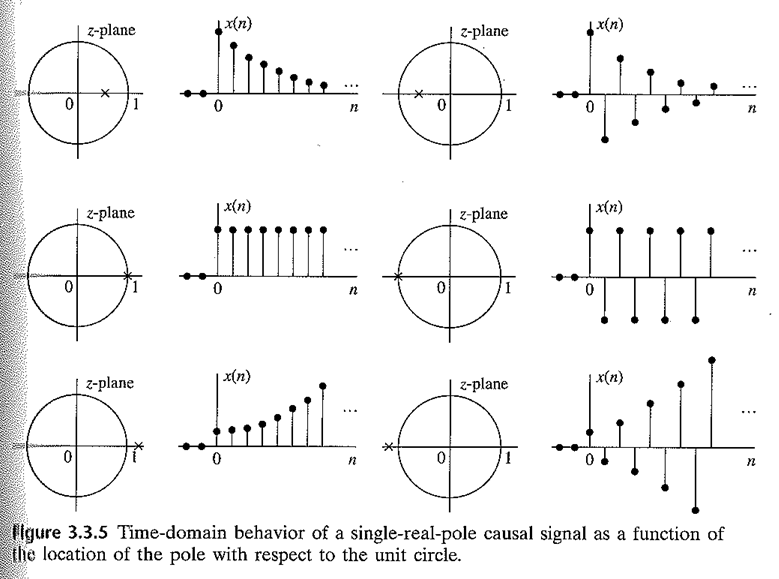
\includegraphics[width=12cm]{singlepole.png}
\end{center}

\vskip 0.2 cm
\noindent
\textbf{Cas 2}. Senyal real amb dos pols reals: $x[n]=n a^nu[n]$, $X(z)=\frac{az^{-1}}{(1-az^{-1})^2}$, ROC=$|z|>|a|$, ($a$ real)
\begin{center}
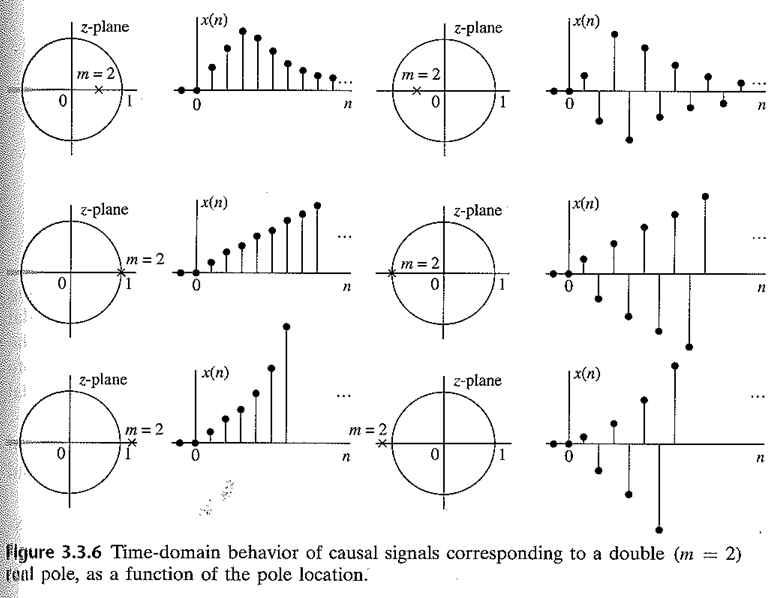
\includegraphics[width=12cm]{doublerealpole.png}
\end{center}

\newpage
\noindent
\textbf{Cas 3}. Senyal real amb un parell de pols complexes conjugats: $x[n]=(a^n \cos(\omega_0 n) ) u[n]$, 
$X(z)=\frac{1-az^{-1}\cos(\omega_0)}{1-2az^{-1}\cos(\omega_0)+a^2z^{-2}}$, ROC=$|z|>|a|$, ($a$ real)
\begin{center}
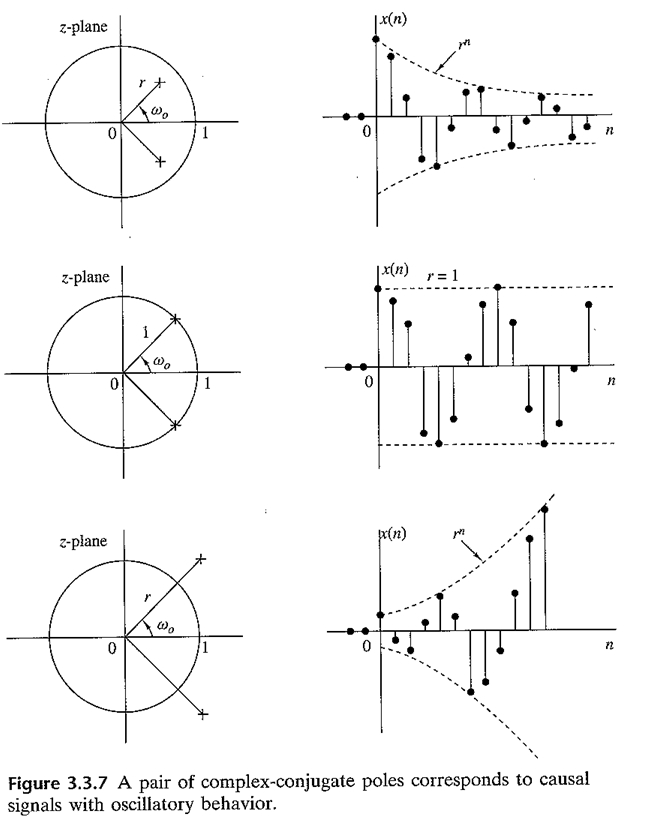
\includegraphics[width=12cm]{doublecomplexpole.png}
\end{center}

\vskip 0.5 cm
\noindent
En general podem afirmar que els senyals causals reals amb els pols a l'interior del \textbf{cercle unitat} ($|z|=1$)
s\'on fitats en amplitud. Si els pols estan a l'exterior del cercle unitat els senyals no s\'on fitats i
si els pols estan damunt el cercle unitat els senyals s\'on fitats si els pols tenen multiplicitat 1.
A m\'es, per al cas de pols dins el cercle unitat el decreixement del senyal \'es m\'es r\`apid com m\'es
a prop de l'origen es troben els pols.

\newpage
\noindent
\textbf{Inversi\'o de transformades Z racionals}

\vskip 0.2 cm
\noindent
L'objectiu \'es trobar $x[n]$ a partir de $X(z)=\frac{B(z)}{A(z)}=
\frac{b_0+b_1z^{-1}+\cdots+b_Mz^{-M}}{1+a_1z^{-1}+\cdots+a_Nz^{-N}}$ i la seva ROC.
El procediment \'es el seg\"uent:

\begin{enumerate}
\item si $M \geq N$ dividim els polinomis fins a trobar una expressi\'o amb la forma seg\"uent:
\[
X(z)=c_0+c_1z^{-1}+\cdots+c_{M-N} z^{-(M-N)}+\frac{B'(z)}{A(z)}
\]

on es compleix que $\frac{B'(z)}{A(z)}=\frac{b^{'}_0+b^{'}_1z^{-1}+\cdots+b^{'}_Kz^{-K}}{1+a_1z^{-1}+\cdots+a_Nz^{-N}}$
amb $K < N$.

El senyal $x_0[n]$ corresponent a $X_0(z)= c_0+c_1z^{-1}+\cdots+c_{M-N} z^{-(M-N)}$ \'es 
$x_0[n]=\{\underline{c_0}, c_1, \cdots, c_{M-N}\}$.

\item si $M < N$ (suposant $a_N \neq 0$):
\begin{enumerate}
\item descomposam la funci\'o racional en factors:
\begin{enumerate}
\item reescrivim $X(z)=\frac{B(z)}{A(z)}$ de la forma 
\[
\frac{X(z)}{z}=\frac{B'(z)}{A'(z)}=\frac{b^{'}_0 z^{N-1} + b^{'}_1 z^{N-2} + \cdots + b^{'}_N z^{N-M-1}}{z^N+a^{'}_1 z^{N-1} + \cdots + a^{'}_N}
\]
\item trobam les arrels de $A'(z)$
\item si totes les arrels s\'on diferents: 
\[
\frac{X(z)}{z}= \frac{A_1}{z-p_1} + \frac{A_2}{z-p_2} + \cdots + \frac{A_N}{z-p_N}
\]
\item si alguna arrel $p_i$ t\'e multiplicitat $k > 1$ la descomposici\'o en factors corresponent a
aquesta arrel \'es
\[
\frac{A_{1i}}{z-p_i} + \frac{A_{2i}}{(z-p_i)^2} + \cdots + \frac{A_{ki}}{(z-p_i)^k}
\]
\item trobam les constants $A_1, \cdots, A_N$ per igualaci\'o amb l'expressi\'o de $\frac{X(z)}{z}$
\end{enumerate}
\item escrivim $X(z)$ de la forma:
\[
X(z)= \frac{A_1}{1-p_1z^{-1}} + \frac{A_2}{1-p_2z^{-1}} + \cdots + \frac{A_{1i}}{1-p_i z^{-1}} + \frac{A_{2i} z^{-1}}{(1-p_i z^{-1})^2} + 
\cdots + \frac{A_N}{1-p_Nz^{-1}}
\]
\item calculam el senyal corresponent a cada sumand de $X(z)$, tenint en compte les seg\"uents propietats:
\[
\begin{array}{c|c|cr}
X(z) & \text{ROC} & x[n] & \\ \hline & & & \\
\frac{1}{1-pz^{-1}} & |z|>|p| & p^n u[n] & \text{(senyal causal)} \\ & & & \\
\frac{1}{1-pz^{-1}} & |z|<|p| & -p^n u[-n-1] & \text{(senyal anticausal)} \\ & & & \\
\frac{A}{1-pz^{-1}}  + \frac{A^*}{1-p^*z^{-1}} & |z|>|p| & 2 |A| r^n \cos(\beta n + \alpha) u[n] & 
A=|A|e^{j\alpha}, \,\, r=|r|e^{j\beta}, \,\, \text{(senyal causal)} \\ & & & \\
\frac{pz^{-1}}{(1-pz^{-1})^2} & |z|>|p| & np^nu[n] & \text{(senyal causal)}
\end{array}
\]

\end{enumerate}

\end{enumerate}


\vskip 0.5 cm
\noindent
\textbf{Exemple}: determinau el sistema causal que t\'e per transformada 
\[
X(z)=\frac{1}{(1+z^{-1})(1-z^{-1})^2}
\]

\vskip 0.3 cm
\noindent
\textbf{Soluci\'o}:
\begin{enumerate}
\item en aquest cas $M=0$ i $N=3$, per tant $M < N$. Reescrivim la transformada de
la forma:
\[
X(z)=\frac{z^3}{(z+1)(z-1)^2} \qquad \Longrightarrow \qquad \frac{X(z)}{z}=\frac{z^2}{(z+1)(z-1)^2}
\]
\item les arrels de $(z+1)(z-1)^2$ s\'on $p_1=-1$ i $p_2=1$ (doble), per tant podem descomposar $X(z)/z$
de la seg\"uent manera:
\[
\frac{X(z)}{z}=\frac{z^2}{(z+1)(z-1)^2}=\frac{A_1}{z+1}+\frac{A_2}{z-1}+\frac{A_3}{(z-1)^2}
\]
\item calculam les constants per comparaci\'o dels numeradors de les expressions anteriors i trobam 
$A_1=\frac{1}{4}$, $A_2=\frac{3}{4}$ i $A_3=\frac{1}{2}$. Per tant:
\[
X(z)=\frac{1}{4} \frac{1}{1+z^{-1}} + \frac{3}{4} \frac{1}{1-z^{-1}} + \frac{1}{2} \frac{z^{-1}}{(1-z^{-1})^2} 
\]
\item mirant les taules de transformades Z habituals trobam les transformades de cada sumand, tenint
en compte que el senyal que buscam \'es causal:
\[
x[n]=\frac{1}{4} (-1)^nu[n] + \frac{3}{4} u[n] + \frac{1}{2} n (1)^n u[n] = 
\left( \frac{1}{4} (-1)^n + \frac{3}{4} + \frac{1}{2} n \right) u[n]
\]
\end{enumerate}

\vskip 1cm
\noindent
\textbf{Inversi\'o de transformades Z descrites com a s\`eries de pot\`encies}

\vskip 0.2 cm
\noindent
Si una $X(z)$ amb una determinada ROC es pot escriure de la seg\"ent manera:
\[
X(z)=\sum_{n=-\infty}^{\infty} c_n z^{-n}
\]
\noindent
i aquesta s\`erie convergeix dins la ROC donada, llavors $x[n]=c_n$, per a tot $n$.

\vskip 0.2 cm
\noindent
Exemples:
\vskip 0.2 cm
\begin{tabular}{l|l|l}
$X(z)$ & ROC & $x[n]$ \\ \hline & & \\
$\frac{1}{1-1.5z^{-1}+0.5z^{-2}}$ & $|z|>1$ & $\{\underline{1}, \frac{3}{2}, \frac{7}{4}, \cdots \}$ \\ \hline & & \\
$\frac{1}{1-1.5z^{-1}+0.5z^{-2}}$ & $|z|<0.5$ & $\{ \cdots, 14, 6, 2, 0, \underline{0} \}$ \\ \hline & & \\
$\log(1+az^{-1})$ & $|z|>|a|$ & $\begin{cases} (-1)^{n+1} \frac{a^n}{n} & \text{si }n \geq 1 \\ \\ 0 & \text{si } n \leq 0 \end{cases}$
\\ & & (Nota: $\log(1+x)=\sum_{n=1}^\infty \frac{ (-1)^{n+1} x^n}{n}$ si $|x|<1$)
\end{tabular}


\newpage
\noindent
\textbf{An\`alisi de sistemes LTI mitjan\c{c}ant la transformada Z}

\vskip 0.3 cm
\noindent
Recordem que la resposta d'un sistema LTI a una entrada $x[n]$ es pot escriure com
\[
y[n]=h[n] * x[n]
\]
\noindent
on $h[n]$ \'es la resposta impulsional del sistema.

\vskip 0.2 cm
\noindent
Aplicant les propietats de la transformada Z podem escriure l'expressi\'o anterior
de la seg\"uent manera:
\[
Y(z)=H(z) X(z)
\]
\noindent
on $X(z)$, $Y(z)$ i $H(z)$ s\'on les transformades Z de $x[n]$, $y[n]$ i $h[n]$, respectivament.
$H(z)$ rep el nom de \textbf{funci\'o de transfer\`encia} del sistema.

\vskip 0.2 cm
\noindent
Si coneixem l'entrada i la sortida del sistema podem calcular $H(z)$:
\[
H(z)=\frac{Y(z)}{X(z)}
\]

\vskip 0.2 cm
\noindent
Si la relaci\'o entre $x[n]$ i $y[n]$ s'expressa mitjan\c{c}ant una equaci\'o en difer\`encies
finites podem calcular $H(z)$ amb la f\`ormula anterior i utilitzant les propietats de la transformada Z.

\vskip 0.2 cm
\noindent
\textbf{Exemple}: determinau la resposta impulsional del sistema causal descrit per la seg\"uent equaci\'o
\[
y[n]=\frac{1}{2}y[n-1]+2x[n]
\]

\vskip 0.2 cm
\noindent
\textbf{Soluci\'o}: 
\begin{enumerate}
\item aplicam la transformada Z als dos membres de l'equaci\'o i aplicam propietats:
\[
Y(z)=\frac{1}{2}z^{-1}Y(z)+2X(z)
\]
\item escrivim la relaci\'o $Y(z)/X(z)$:
\[
Y(z)-\frac{1}{2}z^{-1}Y(z)=2X(z) \qquad \Longrightarrow \qquad H(z)=\frac{Y(z)}{X(z)}=\frac{2}{1-\frac{1}{2}z^{-1}}
\]
\item comparant amb la taula de transformades Z habituals trobam que 
\[
h[n]=2(\frac{1}{2})^n u[n]
\]
\noindent
ja que el sistema \'es causal i per tant $h[n]$ tamb\'e ho \'es.
\end{enumerate}


\vskip 0.5 cm
\noindent
\textbf{Causalitat i estabilitat de sistemes LTI}

\vskip 0.2 cm
\noindent
L'an\`alisi de $H(z)$ permet determinar de manera molt senzilla les caracter\'istiques de
causalitat i estabilitat d'un sistema LTI:
\begin{itemize}
\item Un sistema LTI \'es causal si i nom\'es si la ROC de $H(z)$ \'es l'exterior d'un cercle de
radi $r < \infty$, incloent el punt $z=\infty$.
\item Un sistema LTI \'es estable si i nom\'es si la ROC de $H(z)$ cont\'e el cercle unitat.
\item Un sistema LTI causal \'es estable si i nom\'es si tots els pols de $H(z)$ estan a l'interior 
del cercle unitat. 
\item Un sistema LTI causal amb pols al cercle unitat pot produir una sortida estable 
si el senyal d'entrada i H(z) no tenen pols en com\'u. 
\item La cancel.laci\'o de pols i zeros en l'expressi\'o de $H(z)$ pot produir sistemes 
estables que en la pr\`actica no ho s\'on degut a la imperfecta cancel.laci\'o dels pols i els zeros.
\end{itemize}
 

\end{document}



\documentclass{article}
\usepackage[catalan]{babel}
\usepackage[latin1]{inputenc}   % Permet usar tots els accents i car�ters llatins de forma directa.
\usepackage{enumerate}
\usepackage{amsfonts, amscd, amsmath, amssymb}
\usepackage[pdftex]{graphicx}
\usepackage{longtable}

\setlength{\textwidth}{16cm}
\setlength{\textheight}{24.5cm}
\setlength{\oddsidemargin}{-0.3cm}
\setlength{\evensidemargin}{0.25cm} \addtolength{\headheight}{\baselineskip}
\addtolength{\topmargin}{-3cm}

\newcommand\Z{\mathbb{Z}}
\newcommand\R{\mathbb{R}}
\newcommand\N{\mathbb{N}}
\newcommand\Q{\mathbb{Q}}
\newcommand\K{\Bbbk}
\newcommand\C{\mathbb{C}}

\newcounter{exctr}
\newenvironment{exemple}
{ \stepcounter{exctr} 
\hspace{0.2cm} 
\textit{Exemple  \arabic{exctr}: }
\it
\begin{quotation}
}{\end{quotation}}


\begin{document}

\textbf{\Large Tema 4.An\`alisi de Fourier i mostreig de senyals}

\vskip 0.2 cm
\textbf{\large An\`alisi de Fourier}

Per an\`alisi de Fourier ens referim a un conjunt de t\`ecniques matem\`atiques,
inspirades en els treballs de Joseph Fourier a principis del segle XIX, que
permeten descomposar qualsevol senyal en una suma de senyals sinuso\"idals
de diferents freq\"u\`encies.

Aquesta descomposici\'o \'es \'unica, de manera que es pot caracteritzar qualsevol 
senyal pel conjunt de freq\"u\`encies de les sinusoides que el composen. Per aquest
motiu l'an\`alisi de Fourier rep tamb\'e el nom d'\textbf{an\`alisi freq\"uencial}.

En funci\'o del tipus de senyal a analitzar les eines matem\`atiques per a l'an\`alisi
freq\"uencial varien i reben diferents noms (veure resum en la figura \ref{sumariFourier}):


\begin{description}

\item[Cas 1.] $x$ senyal anal\`ogic (temps continu) peri\`odic, de periode $T$:

\[
\begin{array}{ll}
x(t)=\displaystyle \sum_{k=-\infty}^{\infty} c_k e^{j \frac{2\pi k}{T} t} & \textbf{(s\`erie de Fourier)} \\ \\
c_k=\displaystyle \frac{1}{T} \int_T x(t) e^{-j \frac{2\pi k}{T} t} \, dt &
\end{array}
\]

\noindent
Propietats:
\begin{itemize}
\item An\`alisi freq\"uencial: freq\"u\`encies m\'ultiples de $\frac{1}{T}$.
\item La definici\'o de s\`erie de Fourier nom\'es t\'e sentit si el sumatori 
$\sum_{k=-\infty}^{\infty} c_k e^{j \frac{2\pi k}{T} t}$ convergeix per a tot valor de $t$.
Les \textit{condicions de Dirichlet} garanteixen que la s\`erie existeix per a tots els
valors de $t$:
\begin{enumerate}[i)]
\item $x(t)$ t\'e un nombre finit de discontinu\"itats en cada periode
\item $x(t)$ cont\'e un nombre finit de m\`axims i m\'inims en cada periode
\item $x(t)$ \'es absolutament integrable en un periode: $\int_{T} |x(t)| \, dt < \infty$
\end{enumerate}
Si un senyal no \'es absolutament integrable per\`o verifica que 
$\int_{T} |x(t)|^2 \, dt < \infty$ (senyal d'energia finita), llavors $x(t)$ i la seva s\`erie
de Fourier poden \'esser diferents per a alguns valors de $t$.

En general, tots els senyals peri\`odics d'inter\'es satisfan les condicions de Dirichlet.

\item Si $x(t)$ \'es un senyal real: 
\[
\displaystyle x(t)=c_0+ 2 \sum_{k=1}^\infty |c_k| \cos(\frac{2\pi k}{T} t + \theta_k)
\]
\noindent
on $c_k=|c_k|e^{j\theta_k}$. $|c_0|$ representa el valor mitj\`a del senyal en un periode.

\noindent
Si $x(t)$ \'es real i parell $x(-t)=x(t)$ llavors els coeficients $c_k$ s\'on reals. 
\noindent
Si $x(t)$ \'es real i imparell $x(-t)=-x(t)$ llavors els coeficients $c_k$ s\'on imaginaris purs. 

\item La pot\`encia del senyal $x$ es pot calcular a partir dels coeficients de la seva s\`erie de Fourier
(f\`ormula de Parseval).
(Recordem que l'energia dels senyals peri\`odics \'es infinita):
\[
P=\frac{1}{T} \int_T |x(t)|^2 \, dt = \sum_{k=-\infty}^\infty |c_k|^2
\]
\noindent
La representaci\'o dels valors de $|c_k|^2$ per a cada valor de freq\"u\`encia $\frac{k}{T}$ 
rep el nom d'\textbf{espectre de pot\`encia} o \textbf{densitat espectral de pot\`encia}.
Si el senyal \'es real llavors l'espectre de pot\`encia \'es sim\`etric respecte a l'eix vertical,
ja que $|c_{-k}| =|c_k|$. 


\end{itemize}

\vskip 0.2 cm
\noindent
\textbf{Exemple:} s\`erie de Fourier d'un pols rectangular peri\`odic

\begin{figure}[htbp]
\begin{center}
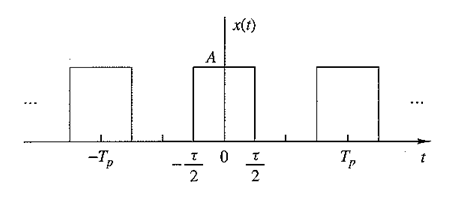
\includegraphics[width=6cm]{polsrectper.png} 
$\qquad$
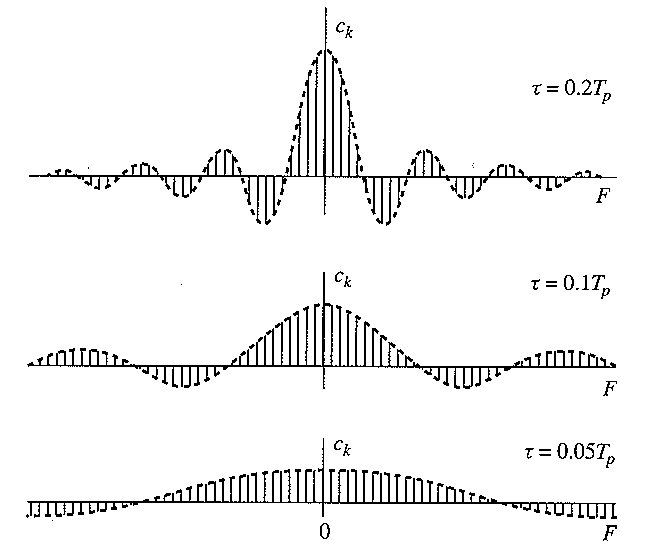
\includegraphics[width=6cm]{sincdiscret1.png} 
\end{center}
\caption{Senyal continu peri\`odic (pols rectangular d'amplada $\tau$) de periode $T_p$ i coeficients de la
seva s\`erie de Fourier per a diferents valors de $\tau$ amb $T_P$ fixat.}
\end{figure}

\newpage

\item[Cas 2.] $x$ senyal anal\`ogic (temps continu) no per�\`odic:

\[
\begin{array}{ll}
x(t)=\displaystyle \int_{-\infty}^{\infty} X(f) e^{j 2\pi f t} \, df &  \\ \\
X(f)=\displaystyle \int_{-\infty}^{\infty} x(t) e^{-j 2\pi f t} \, dt & \textbf{(transformada de Fourier)}
\end{array}
\]

\noindent
Alternativament, aquestes expressions es poden escriure en termes de la freq\"u\`encia angular $\omega=2\pi f$:

\[
\begin{array}{ll}
x(t)=\frac{1}{2\pi} \displaystyle \int_{-\infty}^{\infty} X(\omega) e^{j \omega t} \, d\omega &  \\ \\
X(\omega)=\displaystyle \int_{-\infty}^{\infty} x(t) e^{-j \omega t} \, dt & \textbf{(transformada de Fourier)}
\end{array}
\]

\noindent $X(f)$ rep el nom d'\textbf{espectre del senyal} i tamb\'e es denota com ${\cal F}(x(t))$.
La transformada inversa de Fourier es denota ${\cal F}^{-1}(X(f))=x(t)$.

\noindent
Propietats:
\begin{itemize}
\item An\`alisi freq\"uencial: totes les freq\"u\`encies.

\item La definici\'o de transformada de Fourier nom\'es t\'e sentit si la integral 
$\int_{-\infty}^{\infty} x(t) e^{-j \omega t} \, dt$ convergeix per a tot valor de $t$.
Les \textit{condicions de Dirichlet} garanteixen que la transformada existeix per a tots els
valors de $t$:
\begin{enumerate}[i)]
\item $x(t)$ t\'e un nombre finit de discontinu\"itats finites
\item $x(t)$ cont\'e un nombre finit de m\`axims i m\'inims
\item $x(t)$ \'es absolutament integrable: $\int_{-\infty}^\infty |x(t)| \, dt < \infty$
\end{enumerate}
Si un senyal no \'es absolutament integrable per\`o verifica que 
$\int_{-\infty}^\infty |x(t)|^2 \, dt < \infty$ (senyal d'energia finita), llavors
tamb\'e existeix la seva transformada de Fourier. En aquest cas, a m\'es, es pot assegurar que
tamb\'e existeix la transformada inversa i que ${\cal F}^{-1} {\cal F} x(t)=x(t)$.

\noindent
En la pr\`actica, per a tots els senyals que trobarem en el ``mon real'' podrem calcular
les seves transformades i transformades inverses de Fourier.
\item L'energia del senyal $x$ es pot calcular a partir dels coeficients de la seva transformada de Fourier
(f\`ormula de Parseval):
\[
E=\int_{-\infty}^\infty |x(t)|^2 \, dt = \int_{-\infty}^\infty |X(f)|^2 \, df
\]

S'anomena \textbf{densitat espectral d'energia} a la funci\'o $S_{XX}(f)=|X(f)|^2$.

\item si $x(t)$ \'es un senyal real llavors $|X(-f)|=|X(f)|$ (espectre sim\`etric respecte a l'eix vertical)
i $S_{XX}(-f)=S_{XX}(f)$.


\end{itemize}

\vskip 0.2 cm
\noindent
\textbf{Exemple:} transformada de Fourier d'un pols rectangular

\begin{figure}[htbp]
\begin{center}
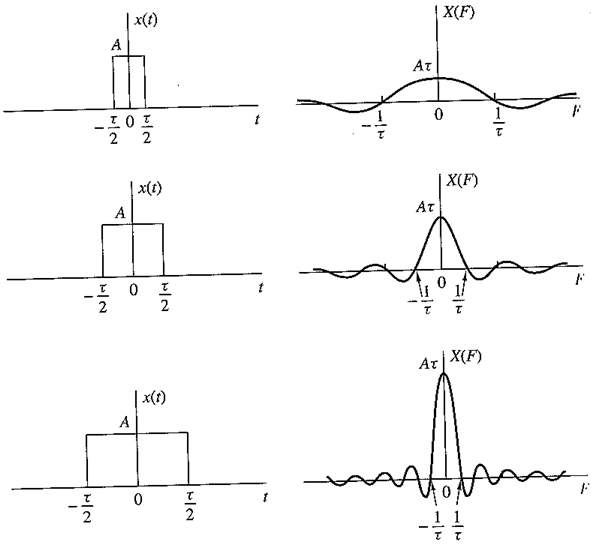
\includegraphics[width=8cm]{polsrectitransfF2.png} 
\end{center}
\caption{Senyal continu no peri\`odic (pols rectangular d'amplada $\tau$) i la
seva transformada de Fourier per a diferents valors de $\tau$.}
\end{figure}


\item[Cas 3.] $x$ senyal digital (temps discret) peri\`odic de periode $N$:

\[
\begin{array}{ll}
x[n]=\displaystyle \sum_{k=0}^{N-1} c_k e^{j \frac{2\pi k}{N} n} \qquad n=0, \cdots, N-1&  \textbf{(s\`erie discreta de Fourier)}\\ \\
c_k=X[k]=\displaystyle \frac{1}{N} \sum_{n=0}^{N-1} x[n] e^{-j \frac{2\pi k}{N} n} \qquad k=0, \cdots, N-1 & 
\textbf{(transformada discreta de Fourier (DFT))}
\end{array}
\]

\noindent
Propietats
\begin{itemize}
\item An\`alisi freq\"uencial: $N$ freq\"u\`encies m\'ultiples de $\frac{1}{N}$ (de $f=0$ fins a $f=\frac{N-1}{N}$).
\item La s\`erie discreta de Fourier sempre es pot calcular.
\item Els coeficients $c_k$ formen una seq\"u\`encia peri\`odica de periode $N$, ja que $c_k=c_{k+N}$.
\item La representaci\'o dels coeficients $c_k$ per a cada valor de $k$ rep el nom d'\textbf{espectre} del senyal.
\item La pot\`encia del senyal $x$ es pot calcular a partir dels coeficients de la seva s\`erie de Fourier
(f\`ormula de Parseval):
\[
P=\frac{1}{N} \sum_{k=0}^{N-1} |x[n]|^2  = \sum_{k=0}^{N-1} |c_k|^2
\]
\noindent
La representaci\'o dels valors de $|c_k|^2$ per a cada valor de freq\"u\`encia $\frac{k}{N}$ 
rep el nom d'\textbf{espectre de pot\`encia} o \textbf{densitat espectral de pot\`encia}.
Si el senyal \'es real llavors l'espectre de pot\`encia \'es sim\`etric respecte a l'eix vertical,
ja que $|c_{-k}| =|c_k|$. 
\end{itemize}

\vskip 0.2 cm
\noindent
\textbf{Exemple:} s\`erie de Fourier d'un pols rectangular discret peri\`odic

\begin{figure}[htbp]
\begin{center}
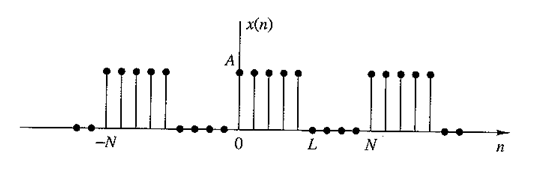
\includegraphics[width=6cm]{polsrectperdiscret.png} 
$\qquad$
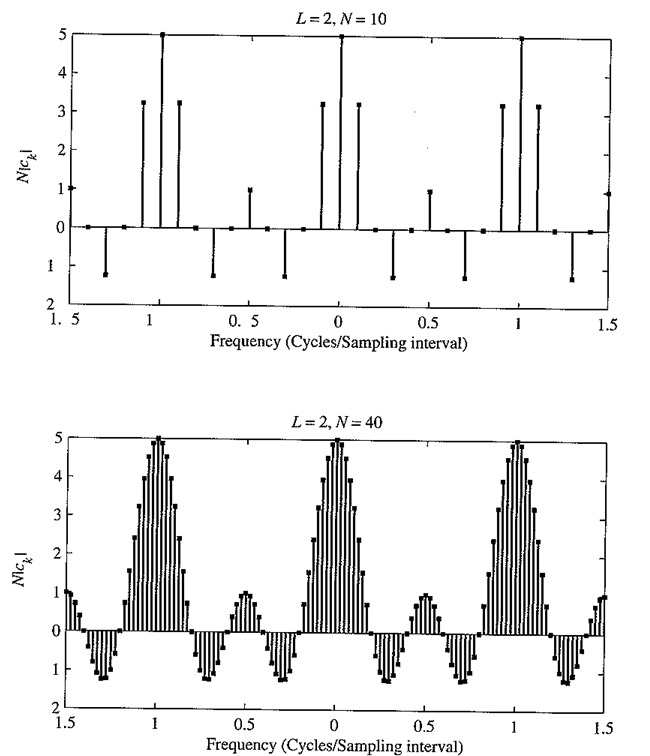
\includegraphics[width=6cm]{sincdiscret.png} 
\end{center}
\caption{Senyal discret peri\`odic (pols rectangular d'amplada $L$) de periode $N$ i coeficients de la
seva s\`erie de Fourier (transformada de Fourier discreta) per a diferents valors de $N$ amb $L$ fixat.
Notem que la transformada discreta \'es tamb\'e peri\`odica amb periode $N$. En la figura de la dreta
l'eix horitzontal representa els valors de freq\"u\`encia $f=k/N$.}
\end{figure}


\item[Cas 4.] $x$ senyal digital (temps discret) no peri\`odic:

\[
\begin{array}{ll}
x[n]=\displaystyle \int_0^1 X(f) e^{j 2 \pi f n} \, df & \\ \\
X(f)=\displaystyle \sum_{n=-\infty}^\infty x[n] e^{-j 2 \pi f n} & \textbf{Transformada de Fourier en temps discret}
\end{array}
\]

\noindent
Alternativament, aquestes expressions es poden escriure en termes de la freq\"u\`encia angular $\omega=2\pi f$:

\[
\begin{array}{ll}
x[n]=\displaystyle \frac{1}{2\pi} \int_0^{2\pi} X(\omega) e^{j \omega n} \, d\omega & \\ \\
X(\omega)=\displaystyle \sum_{n=-\infty}^\infty x[n] e^{-j \omega n} & \textbf{Transformada de Fourier en temps discret}
\end{array}
\]

\noindent
Propietats
\begin{itemize}
\item An\`alisi freq\"uencial: totes les freq\"u\`encies entre $0$ i $1$ (o, de manera equivalent, $\omega \in (0, 2\pi)$).
\item $X(\omega)$ \'es peri\`odica amb periode $2\pi$: $X(\omega+2\pi k)=X(\omega)$, per a tot $k$
\item La transformada de Fourier en temps discret existeix si $x(t)$ \'es absolutament sumable ($\sum_n |x[n]| < \infty$)
o b\'e si \'es d'energia finita ($\sum_n |x[n]|^2 < \infty$).
\item L'energia del senyal $x$ es pot calcular a partir dels coeficients de la seva transformada de Fourier en temps discret
(f\`ormula de Parseval):
\[
E=\sum_{n=-\infty}^\infty |x[n]|^2 = \frac{1}{2\pi} \int_{-\pi}^\pi |X(\omega)|^2 \, d\omega
\]

S'anomena \textbf{densitat espectral d'energia} a la funci\'o $S_{XX}(\omega)=|X(\omega)|^2$.

\item si $x[n]$ \'es un senyal real llavors $|X(-\omega)|=|X(\omega)|$ (espectre sim\`etric respecte a l'eix vertical)
i $S_{XX}(-\omega)=S_{XX}(\omega)$.

\end{itemize}

\vskip 0.2 cm
\noindent
\textbf{Exemple:} transformada de Fourier d'un pols rectangular discret no peri\`odic

\begin{figure}[htbp]
\begin{center}
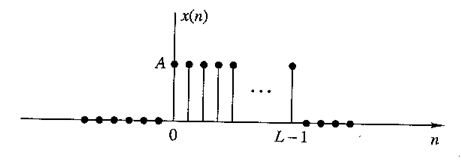
\includegraphics[width=6cm]{polsrectdiscret.png} 
$\qquad$
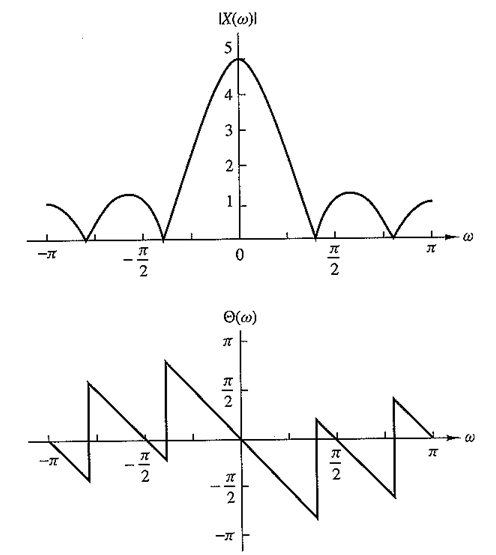
\includegraphics[width=6cm]{polsrectdiscretTF.png} 
\end{center}
\caption{Senyal discret no peri\`odic (pols rectangular d'amplada $L$) i la
seva transformada de Fourier (m\`odul i fase).
Notem que la transformada de Fourier $X(\omega)$ \'es peri\`odica amb periode $2\pi$.}
\end{figure}



\newpage
\noindent
\textbf{Relaci\'o entre la transformada de Fourier en temps discret i la transformada Z}

\noindent
Comparant les definicions de la transformada Z i la transformada de Fourier d'un senyal discret
podem trobar la seg\"uent relaci\'o:

\[
X(\omega)=X(z)|_{z=e^{j\omega}}=\sum_{n=-\infty}^\infty x[n] e^{-j\omega n}
\]

\noindent
Per a que aquesta relaci\'o sigui certa s'han de cumplir que
la transformada Z estigui definida per a $z=e^{j\omega}$, \'es a dir $z=e^{j\omega}$ ha de pert\`anyer a la ROC
de $X(z)$, la qual cosa equival a dir que la ROC de $X(z)$ cont\'e el cercle unitat.

\vskip 0.3 cm
\noindent
\textbf{Propietats de simetria de la transformada de Fourier en temps discret}

\begin{center}
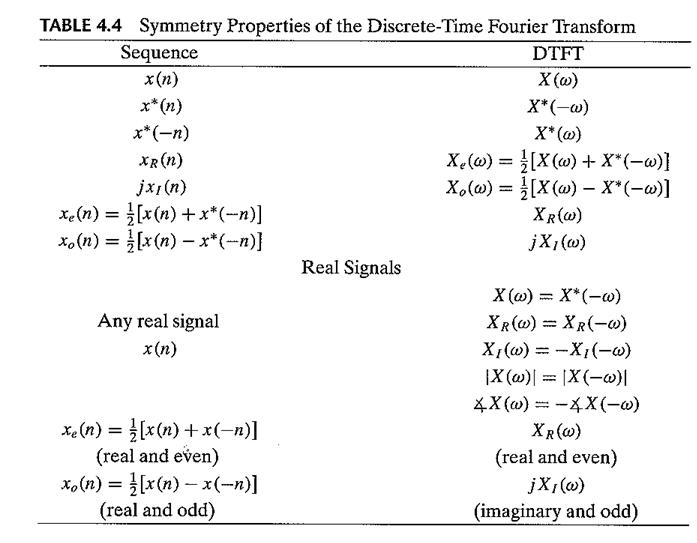
\includegraphics[width=10cm]{tabpropsimetria.png}
\end{center}


\newpage
\noindent
\textbf{Altres propietats de la transformada de Fourier en temps discret}

\begin{center}
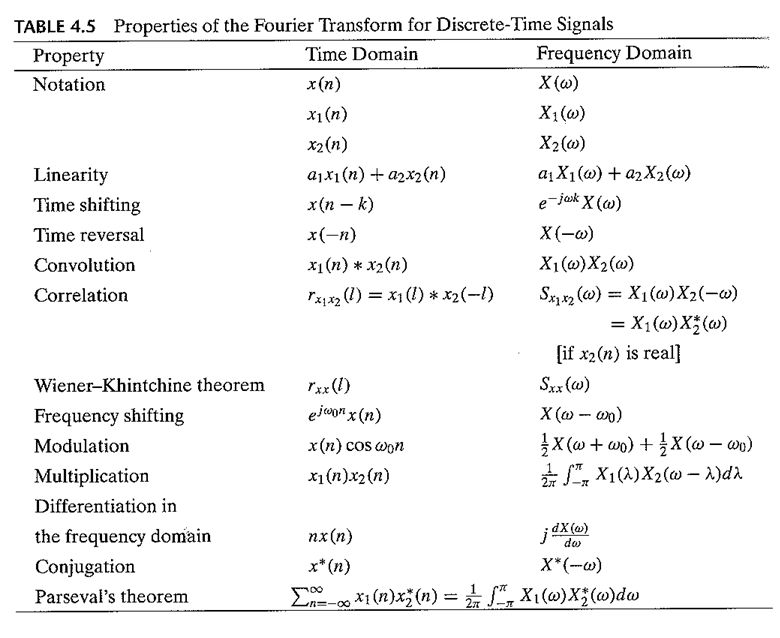
\includegraphics[width=10cm]{tabpropTF.png}
\end{center}

\vskip 0.3 cm
\noindent
\textbf{Parells transformats habituals per a senyals discrets aperi\`odics} 

\begin{center}
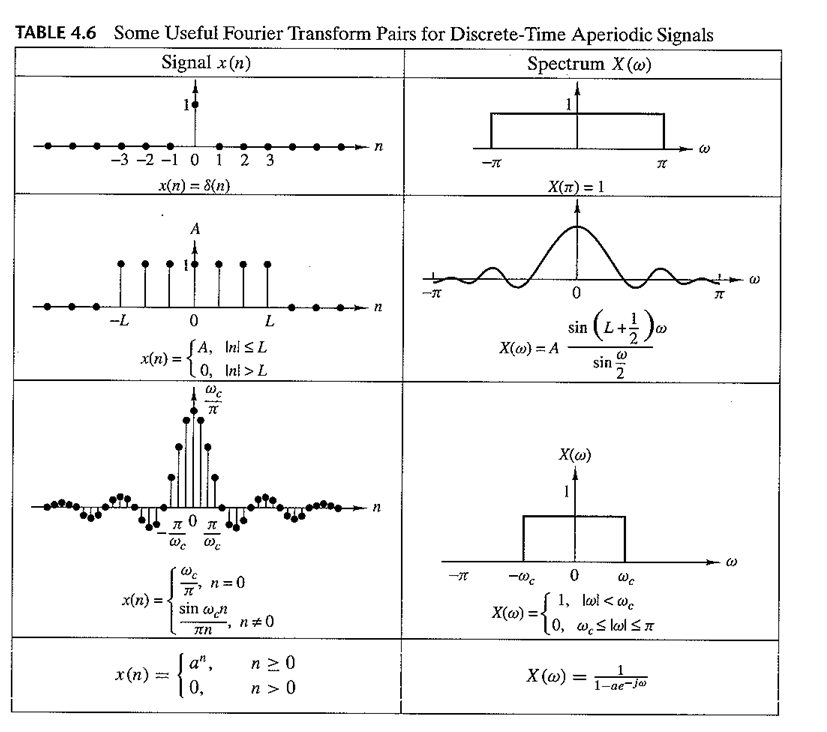
\includegraphics[width=10cm]{tabTFpairs.png}
\end{center}


\end{description}



\begin{figure}[htbp]
\begin{center}
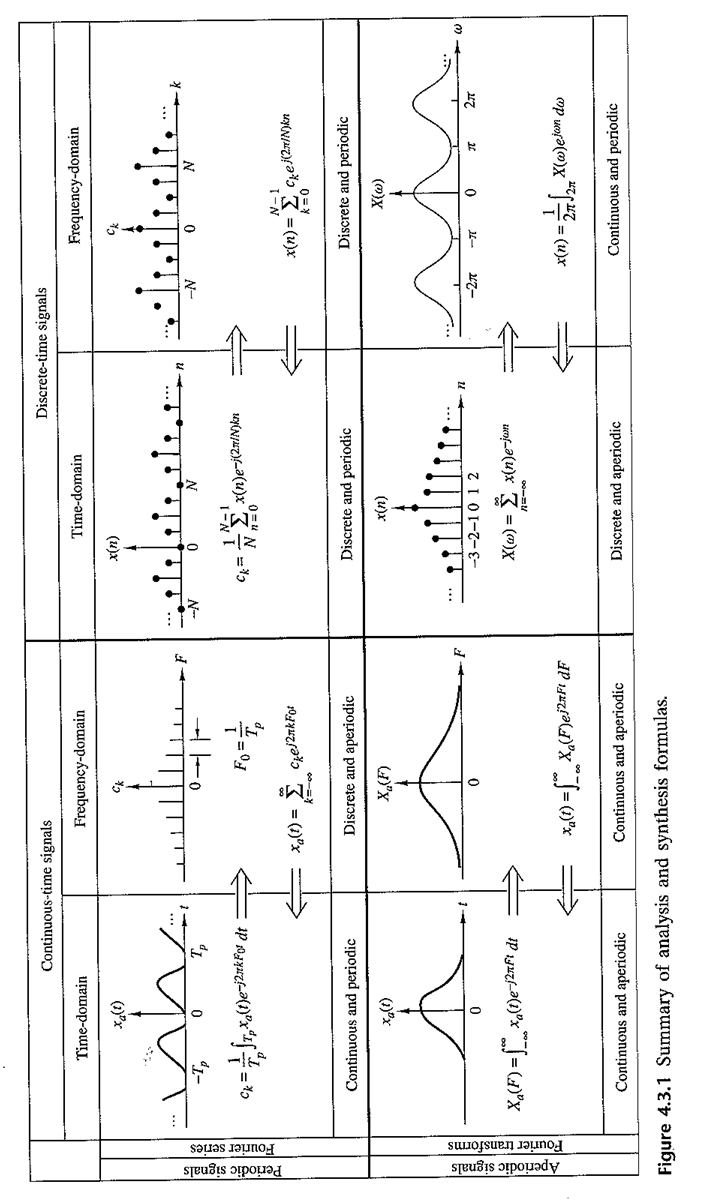
\includegraphics[height=20cm]{sumariTF.png}
\end{center}
\caption{Font: Digital Signal Processing, J. Proakis, D. Manolakis, Pearson Prentice Hall, 2007}
\label{sumariFourier}
\end{figure}




\noindent
\textbf{Relaci\'o entre la Transformada Discreta de Fourier i la Transformada de Fourier en temps discret}

Consideram un senyal discret finit $x[n]$ que pren valors entre $n=0$ i $n=N-1$.
Com es tracta d'un senyal no peri\`odic podem calcular la seva Transformada de Fourier en temps discret:

\[
X(\omega)=\sum_{n=-\infty}^\infty x[n] e^{-j\omega n}=\sum_{n=0}^{N-1} x[n] e^{-j\omega n}
\]

D'altra banda podem considerar l'extensi\'o peri\`odica d'aquest senyal:
\[
x_P[n]=x[n] \qquad \text{si } n=0, \cdots, N-1 \qquad \qquad x_P[n+N]=x_P[n] \quad \text{per a tot } n
\]
\noindent
Observem que per a valors de $n$ entre $0$ i $N-1$ ambd\'os senyals s\'on id\`entics.

\vskip 0.3 cm
\noindent
Aquest nou senyal \'es peri\`odic i per tant podem calcular la seva Transformada Discreta de Fourier:
\[
X_P[k]=\frac{1}{N}\sum_{n=0}^{N-1} x_P[n] e^{-j \frac{2 \pi k}{N} n} =\frac{1}{N}\sum_{n=0}^{N-1} x[n] e^{-j \frac{2 \pi k}{N} n} 
\]

\vskip 0.3 cm
\noindent
Ens demanam per la relaci\'o entre aquestes dues transformades. Comparant les expressions obtingudes observam que:
 
\[
X_P[k]=\frac{1}{N}X(\frac{2\pi k}{N})
\]

\'es a dir, la DFT \'es una versi\'o discreta i reescalada de la Transformada de Fourier del senyal discret.


\vskip 0.3 cm
La conclusi\'o del raonament anterior \'es que \'es possible con\`eixer, de manera aproximada, 
la transformada de Fourier d'un senyal discret a partir de la DFT de la seva versi\'o perioditzada.
En la pr\`actica \'es molt m\'es f\`acil calcular la DFT que la transformada de Fourier, ja que existeixen
algoritmes r\`apids de c\`alcul (anomenats FFT: \textit{Fast Fourier Transform}), amb la ventatja
que el resultat \'es un senyal discret que pot \'esser enmagatzemat en l'ordinador. Per aquest motiu
normalment es calcula la DFT i a partir d'ella es dedueixen propietats de la Transformada de Fourier del senyal.


\vskip 0.4 cm
\noindent
\textbf{Exemple:} comparaci\'o de la transformada de Fourier de $x[n]=a^n u[n]$ (amb $a=0.8$) i la seva transformada
discreta de Fourier (figures \ref{exTFDFT1} i \ref{exTFDFT2}).

\begin{figure}[htbp]
\begin{center}
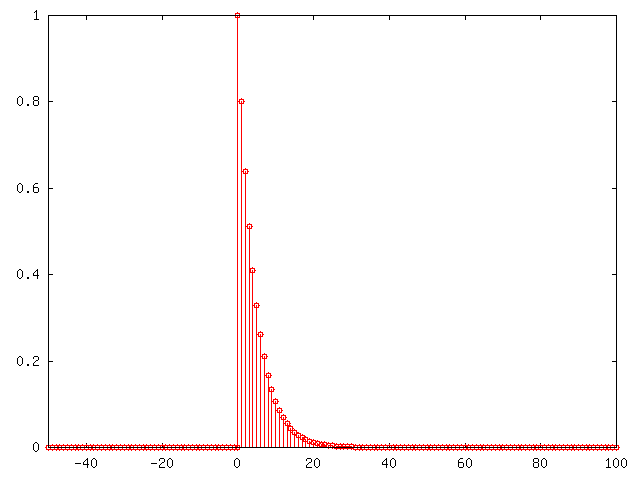
\includegraphics[width=6cm]{signal0_T4.png} 
$\qquad$
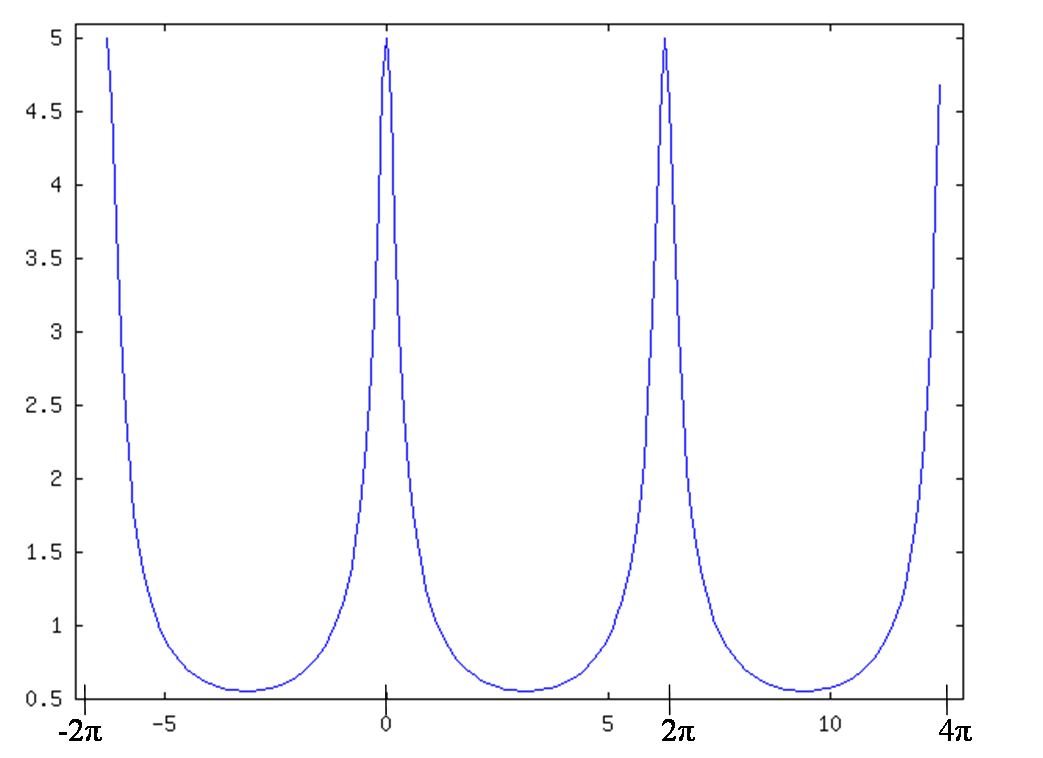
\includegraphics[width=6cm]{TFsignal0bis_T4.png} 
\end{center}
\caption{Senyal discret no peri\`odic i la seva transformada de Fourier .
Notem que la transformada de Fourier $X(\omega)$ \'es peri\`odica amb periode $2\pi$.}
\label{exTFDFT1}
\end{figure}

\begin{figure}[htbp]
\begin{center}
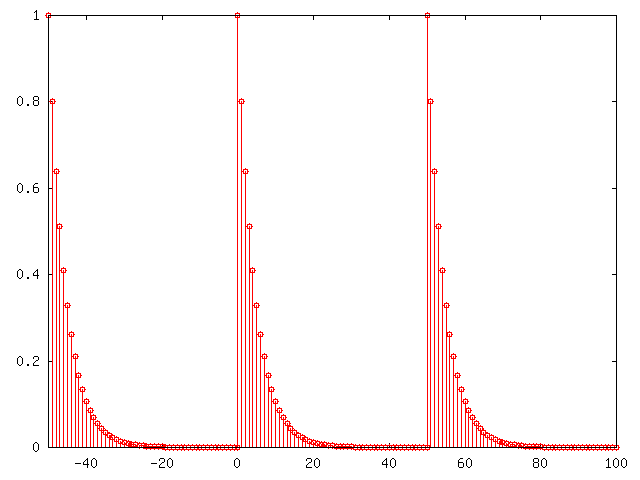
\includegraphics[width=6cm]{signal0P_T4.png} 
$\qquad$
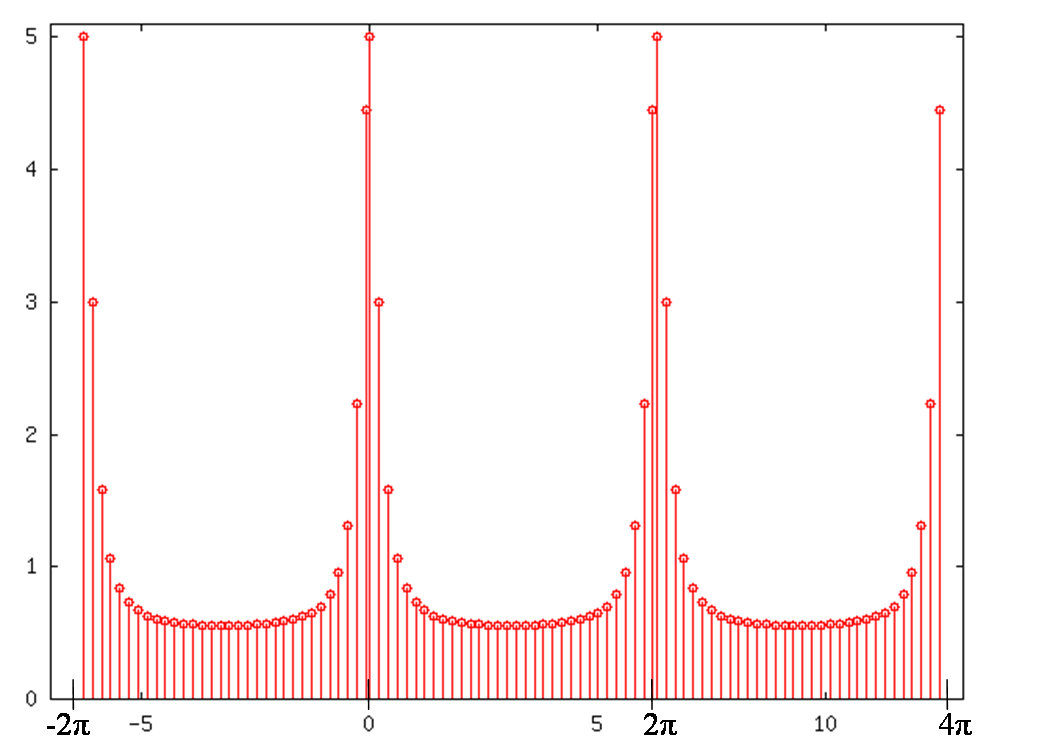
\includegraphics[width=6cm]{TFsignal0Pbis_T4.png} 
\end{center}
\caption{Senyal discret perioditzat (periode $N=50$) i coeficients de la seva s\`erie de Fourier (transformada discreta de Fourier).
Notem que la DFT \'es un versi\'o discreta de la transformada de Fourier del senyal no peri\`odic. La dist\`ancia
entre les mostres \'es $\frac{2\pi}{N}$.}
\label{exTFDFT2}
\end{figure}




\newpage
\textbf{\large Mostreig de senyals}

En aquesta secci\'o estudiam el proc\'es de mostreig de senyals. L'objectiu del mostreig
\'es representar amb un nombre discret de valors (\textit{mostres}) un senyal anal\`ogic (temps continu)
o b\'e representar amb un nombre menor de mostres un senyal digital (temps discret).
Estudiarem el proc\'es de mostreig tant des del punt de vista temporal com des del punt de vista freq\"uencial
i establirem quines condicions ha de verificar el proc\'es per fer possible la recuperaci\'o del senyal
mostrejat original a partir de les seves mostres.


\vskip 0.3 cm
\noindent
\textbf{Mostreig de senyals anal\`ogics}

La figura \ref{figmostreig} il.lustra el proc\'es de mostreig d'un senyal anal\`ogic. El senyal discret obtingut
$x[n]$ \'es igual al senyal original $x_a(t)$ per als valors de $t=nT$, on $T$ rep el nom de \textbf{periode de
mostreig}: $x[n]=x_a(nT)$.

\begin{figure}[htbp]
\begin{center}
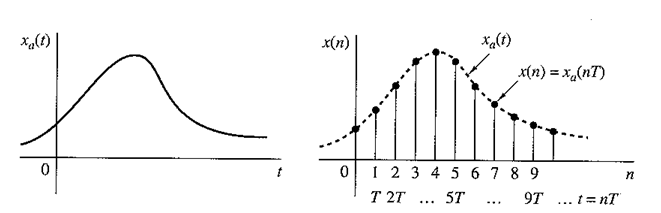
\includegraphics[width=8cm]{figmostreig.png}
\end{center}
\caption{Mostreig d'un senyal continu amb un periode de mostreig $T$.}
\label{figmostreig}
\end{figure}

\vskip 0.2 cm
\noindent
\textbf{Freq\"u\`encies de senyals continus i de senyals discrets}

Per a estudiar el proc\'es de mostreig des del punt de vista freq\"uencial calcularem les transformades de
Fourier de $x_a(t)$ i $x[n]$ aplicant les f\`ormules estudiades en les seccions anteriors (casos 2 i 4, respectivament),
per\`o cal tenir en compte que les ``freq\"u\`encies'' a les quals fan refer\`encia les f\`ormules representen
magnituds diferents en el cas continu i en el cas discret.

En el cas continu la freq\"u\`encia representa el \textit{nombre de cicles per segon} o \textit{hertz} (Hz) (veure la 
Figura \ref{figfreq}-esquerra).


En el cas continu la freq\"u\`encia representa el \textit{nombre de cicles per mostra} (veure la 
Figura \ref{figfreq}-dreta).


\begin{figure}[htbp]
\begin{center}
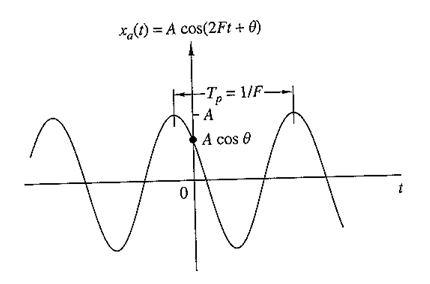
\includegraphics[width=6cm]{ciclessegon.png}
$\qquad$
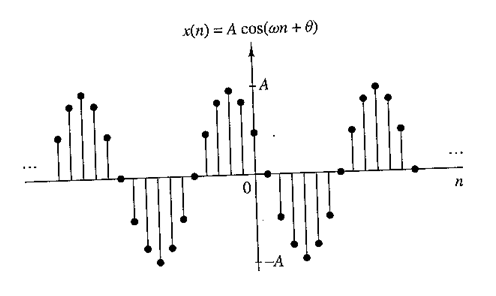
\includegraphics[width=6cm]{ciclesmostra.png}
\end{center}
\caption{Difer\`encia entre la freq\"u\`encia d'un senyal continu (esquerra) i la d'un senyal discret (dreta).}
\label{figfreq}
\end{figure}


Per distingir ambdues magnituds, a partir d'ara utilitzarem la lletra $F$ per denotar la freq\"u\`encia 
d'un senyal continu i $f$ per denotar la d'un senyal discret
\footnote{Tamb\'e utilitzarem la notaci\'o $\Omega$ i $\omega$ per distingir entre freq\"u\`encia angular
dels senyals continus i dels senyals discrets, respectivament}. La relaci\'o entre ambues freq\"u\`encies \'es
$F=\frac{f}{T}$.

Amb aquesta nova notaci\'o les f\`ormules per al c\`alcul de les transformades de Fourier de $x_a(t)$ i $x[n]$
s\'on:


\[
\begin{array}{lcl}
x_a(t)=\displaystyle \int_{-\infty}^{\infty} X(_aF) e^{j 2\pi F t} \, dF  & $\qquad$ &
X_a(F)=\displaystyle \int_{-\infty}^{\infty} x_a(t) e^{-j 2\pi F t} \, dt \\ \\ 
x[n]=\displaystyle \int_0^1 X(f) e^{j 2 \pi f n} \, df  & $\qquad$ &
X(f)=\displaystyle \sum_{n=-\infty}^\infty x[n] e^{-j 2 \pi f n} 
\end{array}
\]


On s'ha de tenir en compte que si $F=\frac{f}{T}$, llavors $X(f)=X(FT)$.


\vskip 0.2 cm
\noindent
\textbf{Relaci\'o entre els espectres de $x_a(t)$ i $x[n]$}
La relaci\'o entre les transformades $X_a$ i $X$ v\'e donada per la seg\"uent expressi\'o:

\[
X(FT)=\frac{1}{T} \sum_{k=-\infty}^\infty X_a(F+\frac{k}{T})
\]

\noindent
\'Es a dir, la transformada del senyal discret s'obt\'e com la superposici\'o de transformades del senyal
continu despla\c{c}ades en freq\"u\`encia a intervals regulars $\frac{1}{T}$.
La figura \ref{exmostreig} il.lustra l'efecte del mostreig en l'espectre d'un senyal.

\vskip 0.2cm
\noindent
La relaci\'o entre $X_a$ i $X$ es pot deduir a partir de les f\`ormules de les transformades descrites en les
seccions anteriors (casos 2 i 4, respectivament). Alternativament, es pot obtenir la relaci\'o entre
aquestes transformades fent us de la versi\'o continua $\hat{x}(t)$ del senyal discret $x[n]=x_a(nT)$, que es
defineix com:
\[
\hat{x}(t)=x_a(t) \cdot \sum_{n=-\infty}^\infty \delta(t-nT)
\]

\noindent
on el sumatori $\sum_{n=-\infty}^\infty \delta(t-nT)$ rep del nom de \textbf{tren de deltes}. $\delta(t)$
es defineix de manera que $\int_{-\infty}^\infty f(t) \delta(t-t_0) \, dt = f(t_0)$ per a qualsevol funci\'o $f(t)$.
Amb aquesta definici\'o es verifica que $\hat{X}(F)=X(FT)$. A m\'es es pot comprovar que $\hat{X}(F)=\frac{1}{T} \sum_{k=-\infty}^\infty X_a(F+\frac{k}{T})$.

\begin{figure}[htbp]
\begin{center}
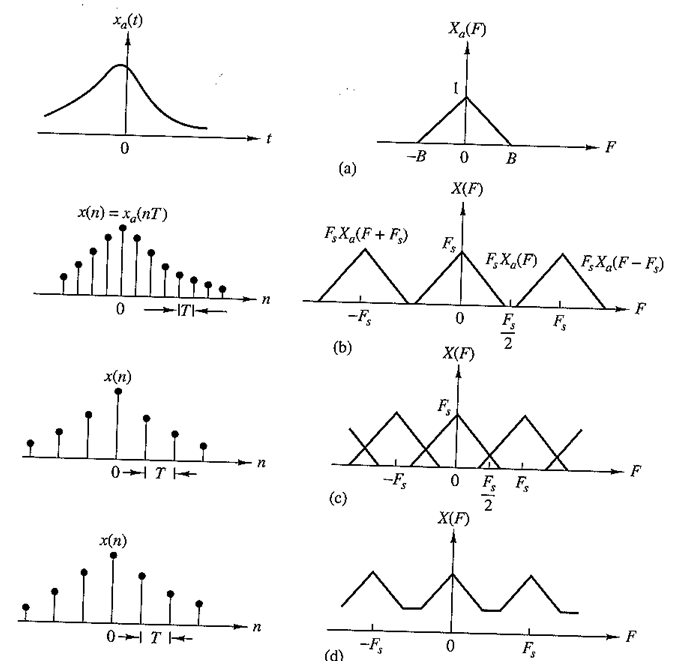
\includegraphics[height=8cm]{exmostreig.png}
\end{center}
\caption{(a) Senyal original i el seu espectre. Notem que el senyal t\'e amplada de banda limitada i que l'espectre
s'anul.la quan $|F|>B$. (b) Senyal mostrejat amb un periode de mostreig $T$ tal que $T < \frac{1}{2B}$ i el seu espectre.
(c) Senyal mostrejat amb un periode de mostreig $T$ tal que $T > \frac{1}{2B}$ i proc\'es de formaci\'o del seu espectre.
(d) Senyal mostrejat amb un periode de mostreig $T$ tal que $T > \frac{1}{2B}$ i el seu espectre.}
\label{exmostreig}
\end{figure}

\vskip 0.3 cm
\noindent
\textbf{Teorema del mostreig (teorema de Shannon-Whitaker)}

Ens demanam en aquesta secci\'o si \'es possible recuperar el senyal continu original a partir de la 
seva versi\'o mostrejada. La resposta \'es s\'i, sempre que la relaci\'o entre l'amplada de banda del
senyal original i la freq\"u\`encia de mostreig sigui l'adequada.
Observant la figura \ref{exmostreig} podem deduir quina \'es aquesta condici\'o:
\renewcommand{\labelitemi}{-}
\begin{itemize}
\item Si $T$ \'es massa gros (\'es a dir, la freq\"u\`encia de mostreig $F_m=\frac{1}{T}$ 
\'es massa petita) les repeticions de l'espectre original es solapen (aquest fen\`omen
rep el nom d'\textbf{aliasing}) (veure (c))
i \'es impossible identificar l'espectre original en l'espectre resultant (veure (d)).
\item En canvi, si $T$ \'es suficientment petit (\'es a dir, $F_m$ \'es suficientment gros), llavors
s\'i es possible identificar l'espectre original en l'espectre resultant (veure (b)).
\end{itemize}

La condici\'o que ha de cumplir la freq\"u\`encia de mostreig per a poder recuperar el senyal original
a partir del mostrejat s'anomena \textbf{condici\'o de Nyquist}, i la freq\"u\`encia m\'inima
de mostreig rep el nom de \textbf{freq\"u\`encia de Nyquist} ($F_N$):
\[
F_m > 2B \qquad \text{per tant} \qquad F_N=2B
\]

En cas que un senyal hagi estat mostrejat satisfent la condici\'o de Nyquist, el \textbf{teorema del
mostreig} ens diu com obtenir el senyal original a partir del mostrejat: 
\begin{itemize}
\item Definim $X_{\Pi}(F)=X(FT) \cdot \Pi(\frac{F}{F_m/2})$, on 
$\Pi(\frac{F}{F_m/2})=\begin{cases} 1 & \text{ si } |F| \leq F_m/2 \\ 0 & \text{altrament} \end{cases}$
\item Si es verifica la condici\'o de Nyquist llavors $X_{\Pi}(F)=\frac{1}{T}  \cdot X_a(F)$ 
\item Calculam $x_a(t)$ com la transformada inversa de $T \cdot X_{\Pi}(F)$:
\[
x_a(t)=T \cdot \int_{-\infty}^\infty X_{\Pi}(F) e^{j 2 \pi F t} \, dF
\]
\item El resultat del c\`alcul d\'ona:
\[
x_a(t)=\sum_{n=-\infty}^\infty x[n] \frac{\sin(\frac{\pi(t-nT)}{T})}{\frac{\pi(t-nT)}{T}}=
\sum_{n=-\infty}^\infty x[n] \cdot \mathrm{sinc}(\frac{\pi(t-nT)}{T})
\]
\noindent
on $\mathrm{sinc}(x)=\frac{\sin x}{x}$.
\end{itemize}

El proc\'es de reconstrucci\'o del senyal original a partir de les seves mostres s'il.lustra 
a les figures \ref{exrecons1} i \ref{exrecons2}. En cas que el senyal mostrejat no satisfaci les condicions de Nyquist
el senyal reconstru\"it \'es diferent de l'original (figura \ref{exmalarecons}).

\begin{figure}[htbp]
\begin{center}
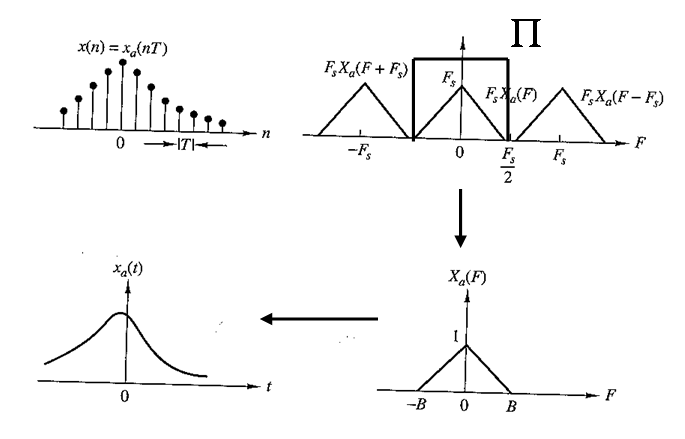
\includegraphics[width=8cm]{exrecons1.png}
\end{center}
\caption{Reconstrucci\'o del senyal anal\`ogic a partir d'un senyal digital mostrejat correctament}
\label{exrecons1}
\end{figure}

\begin{figure}[htbp]
\begin{center}
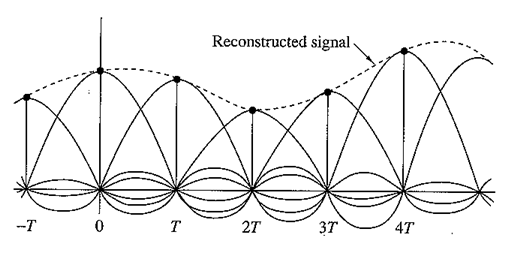
\includegraphics[width=6cm]{exrecons2.png}
\end{center}
\caption{Il.lustraci\'o del proc\'es de reconstrucci\'o del senyal anal\`ogic a partir de les
seves mostres utilitzant la f\`ormula del teorema del mostreig.}
\label{exrecons2}
\end{figure}

\begin{figure}[htbp]
\begin{center}
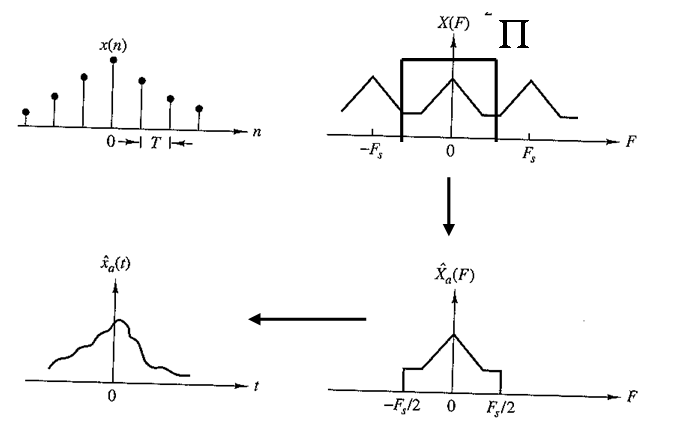
\includegraphics[width=8cm]{exmalarecons.png}
\end{center}
\caption{Dalt, senyal mostrejat sense cumplir la condici\'o de Nyquist i el seu espectre.
Baix, a la dreta, $X_{\Pi}(F)$ corresponent al senyal anterior. Esquerra, reconstrucci\'o del
senyal a partir de $X_{\Pi}(F)$. Comparau amb la figura \ref{exrecons1}.}
\label{exmalarecons}
\end{figure}


\vskip 0.3 cm
\noindent
\textbf{Mostreig de senyals discrets (delmat)}

Volem estudiar el senyal $x_M[n]=x[Mn]$, on $M$ \'es un enter positiu (veure exemple a la figura \ref{exmostreigdiscret}).
El resultat del mostreig \'es un nou senyal discret equivalent a mostrejar el senyal anal\`ogic
original amb un periode de mostreig $MT$ ($T$ \'es el periode de mostreig original).
A nivell freq\"uencial, es pot calcular l'espectre de $x_M[n]$ a partir del de $x[n]$:
\[
X_M(f)=\frac{1}{M} \sum_{k=0}^{M-1} X(\frac{f}{M}-\frac{k}{M})
\]
Observam que el resultat del mostreig \'es un apropament de les repeticions de l'espectre del senyal
anal\`ogic original. Si $M$ \'es massa gros s'arriba a produir aliasing.

\begin{figure}[htbp]
\begin{center}
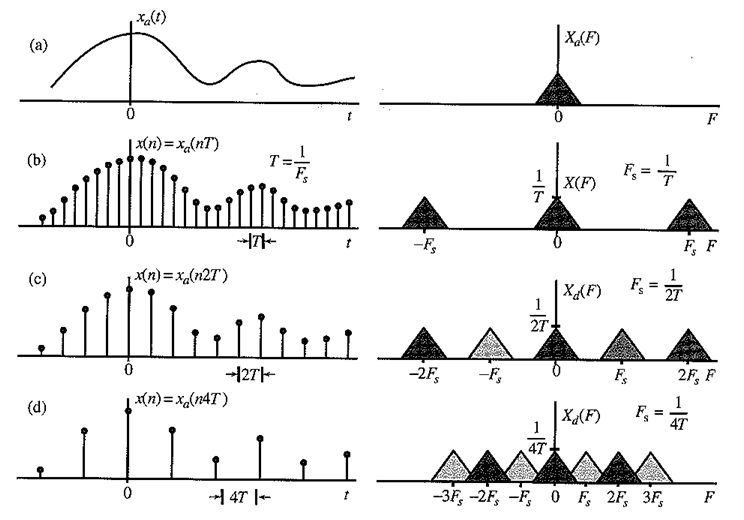
\includegraphics[width=8cm]{exmostreigdiscret.png}
\end{center}
\caption{Exemples de delmat d'un senyal discret}
\label{exmostreigdiscret}
\end{figure}


\vskip 0.5 cm
\noindent
\textbf{\large Processament digital de senyals anal\`ogics}

Considerem un senyal anal\`ogic $x_a(t)$ que es processa amb un sistema ${\cal T}_a$ per donar
com a sortida el senyal $y_a(t)$.

\begin{center}
\begin{minipage}{6cm} 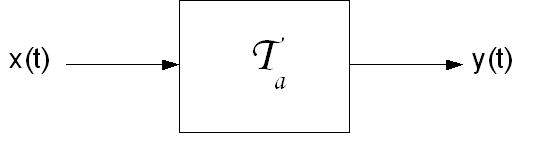
\includegraphics[width=6cm]{sistemaanalogic.png}\end{minipage}
\end{center}

Considerem ara la versi\'o discreta del senyal: $x[n]=x_a(nT)$.

\noindent
\textbf{Propietat:} 

\noindent
Si ${\cal T}_a$ \'es un sistema LTI i 
$T$ \'es un periode de mostreig que satisf\`a la condici\'o de Nyquist llavors es pot trobar
un sistema digital ${\cal T}$ LTI amb funci\'o de transfer\`encia $H(f)$ tal que la
seva sortida $y[n]$ \'es la versi\'o discreta del senyal $y_a(t)$. Es diu en aquest cas
que els sistemes ${\cal T}_a$ i ${\cal T}$ s\'on equivalents.

\vskip 0.3 cm
\noindent
La relaci\'o entre ${\cal T}_a$ i ${\cal T}$ es pot representar amb el seg\"uent diagrama de blocs:

\begin{center}
\begin{minipage}{10cm} 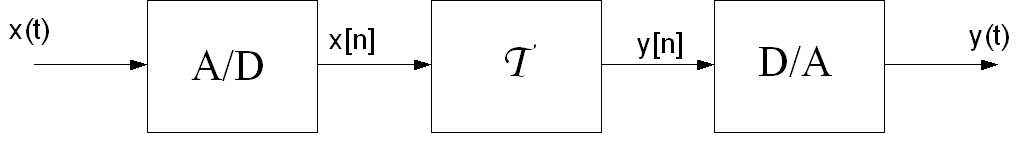
\includegraphics[width=10cm]{sistemadigital.png}\end{minipage}
\end{center}

\noindent
on els blocs \textbf{A/D} i \textbf{D/A} representen els processos de conversi\'o 
d'\textit{anal\`ogic a digital} i de \textit{digital a anal\`ogic}, respectivament. 
En la seva versi\'o m\'es simple aquest processos es poden representar gr\`aficament
amb els seg\"uents diagrames de blocs:

\begin{figure}[htbp]
\begin{center}
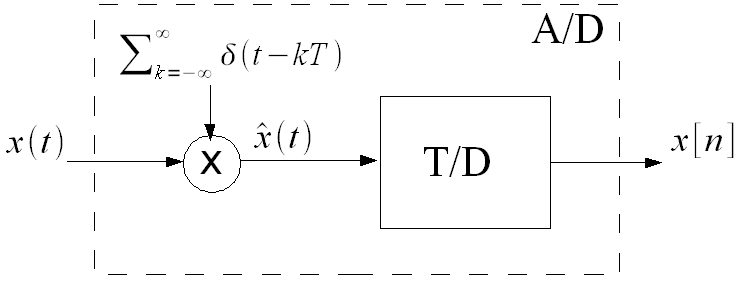
\includegraphics[width=7.5cm]{AD.png}
$\qquad$
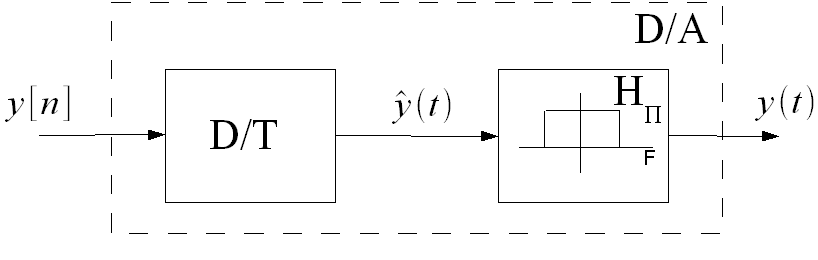
\includegraphics[width=7.5cm]{DA.png}
\end{center}
\end{figure}

El proc\'es de conversi\'o d'anal\`ogic a digital es pot descriure, de manera ideal, en dues etapes: el producte
del senyal anal\`ogic per un tren de deltes i la conversi\'o del resultat (bloc \textbf{T/D}) en la seva versi\'o 
discreta. Processos com la quantificaci\'o i codificaci\'o dels valors del senyal no es tenen en compte.

\vskip 0.3 cm
El proc\'es de conversi\'o de digital a anal\`ogic es pot descriure, de manera ideal, en dues etapes:
el pas a la versi\'o cont\'inua del senyal discret, expressat com a tren de deltes (bloc \textbf{D/T})
i eliminaci\'o de les repeticions de la transformada (bloc \textit{filtre passa-baix}, amb funci\'o de
transfer\`encia $H_{\Pi}(F)$). 

\vskip 0.3 cm
\noindent
La seg\"uent figura mostra dos exemples de conversi\'o D/A i A/D:

\begin{figure}[htbp]
\begin{center}
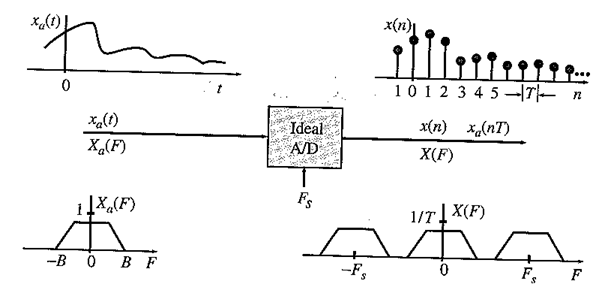
\includegraphics[width=7cm]{exAD.png}
$\qquad$ $\quad$
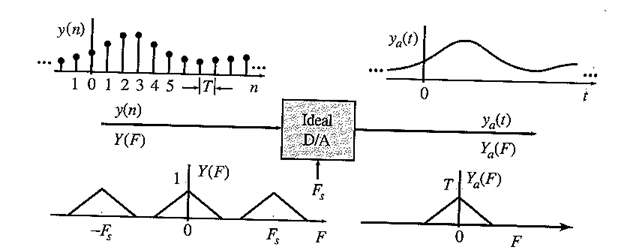
\includegraphics[width=7.5cm]{exDA.png}
\end{center}
\end{figure}


La transformada de Fourier del senyal de sortida $Y_a(F)$ es pot escriure en funci\'o de tots els blocs
del sistema de la seg\"uent manera:

\[
Y_a(F)=H_{\Pi}(f) \cdot H(FT) \cdot \frac{1}{T} \sum_{k=-\infty}^\infty X_a(F-\frac{k}{T})=H(FT) \cdot X_a(F)
\]


\vskip 2cm
\noindent
\textbf{Nota:} la majoria de figures d'aquest cap\'itol s'han tret de Digital Signal Processing, J. Proakis, D. Manolakis, Pearson Prentice Hall, 2007.



\end{document}


\part{}

En este m�dulo avanzamos en el estudio de la Estad�stica Descriptiva con el
estudio de las relaciones entre varias variables estad�sticas.
Al igual que en m�dulo anterior se explica c�mo resolver los problemas con
la ayuda de aplicaciones inform�ticas.

En la segunda parte del m�dulo se dan los fundamentos de Probabilidad necesarios
para el estudio de la Estad�stica Inferencial.

\documentclass{article}
\usepackage{enumerate}
\usepackage{graphicx}
\usepackage{amsfonts, amscd, amsmath, amssymb}

\oddsidemargin -0.3cm
\evensidemargin 0cm
\textwidth 16.5cm
\textheight 21cm

\def\N{\mathbb N}
\def\Z{\mathbb Z}
\def\R{\mathbb R}
\def\C{\mathbb C}

\title{Processament d'imatges}
\date{}

\begin{document}

\maketitle
\tableofcontents

\section{Equalitzaci\'o d'histograma}

\section{Filtratge freq\"uencial}

\section{Filtratge amb m\`ascares}

\section{Filtres morfol\`ogics}

\section{Filtratge i equacions en derivades parcials}

\subsection{Filtratge gaussi\`a i equaci\'o de la calor}

\subsection{Filtratge no lineal}

\end{document} 

\part{}

En este m�dulo se estudian las t�cnicas b�sicas de la Estad�stica Inferencial,
que permiten conocer el grado de fiabilidad de la generalizaci�n de
los datos obtenidos mediante la Estad�stica Descriptiva a conjuntos de datos
mayores.

\end{document}
